\chapter{图像分割}\label{ux7b2cux4e5dux7ae0-ux56feux50cfux5206ux5272}

\section{图像分割算法分类?}\label{ux56feux50cfux5206ux5272ux7b97ux6cd5ux5206ux7c7b}

图像分割是预测图像中每一个像素所属的类别或者物体。基于深度学习的图像分割算法主要分为两类:

\textbf{1.语义分割}

为图像中的每个像素分配一个类别,如把画面中的所有物体都指出它们各自的类别。

\begin{figure}
\centering
%\includegraphics{./img/ch9/Semantic-01.png}
%\caption{}
\end{figure}

\textbf{2.实例分割}

与语义分割不同,实例分割只对特定物体进行类别分配,这一点与目标检测有点相似,但目标检测输出的是边界框和类别,而实例分割输出的是掩膜(mask)和类别。

\begin{figure}
\centering
%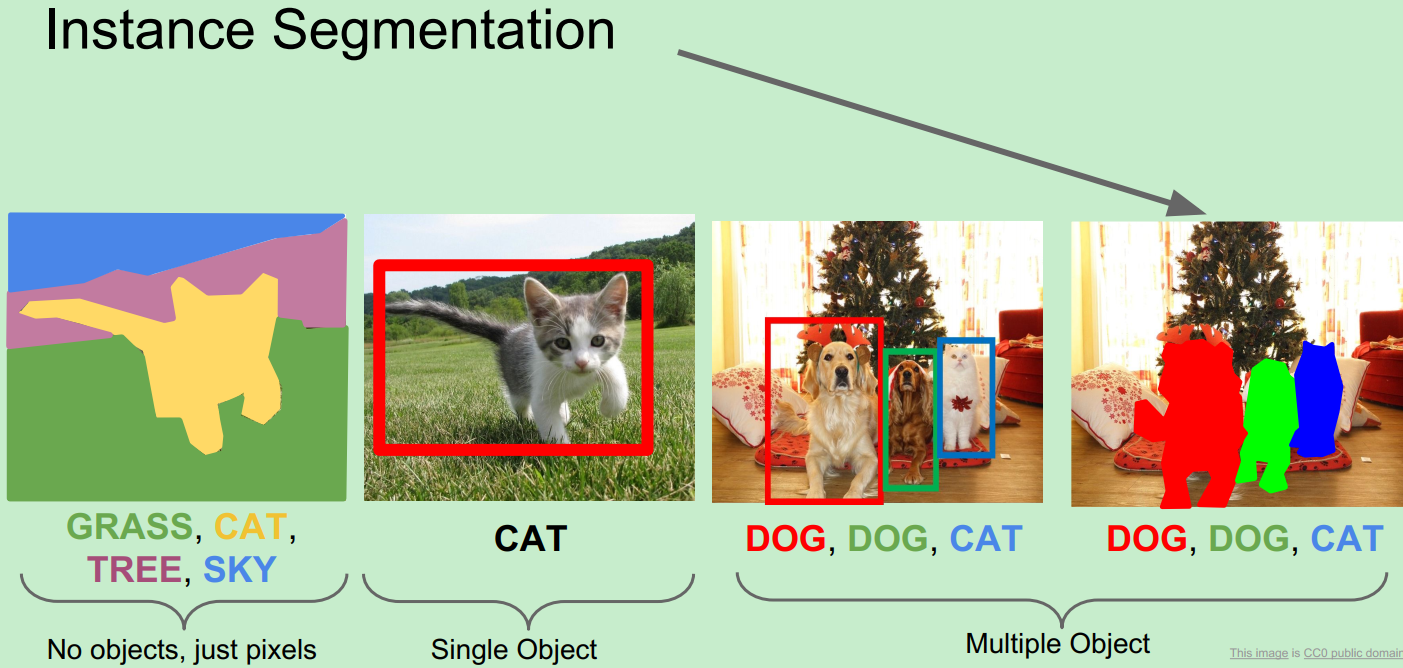
\includegraphics{./img/ch9/Instance-01.png}
%\caption{}
\end{figure}

\section{9.2
传统的基于CNN的分割方法缺点?}\label{ux4f20ux7edfux7684ux57faux4e8ecnnux7684ux5206ux5272ux65b9ux6cd5ux7f3aux70b9}

传统的基于CNN的分割方法:为了对一个像素分类,使用该像素周围的一个图像块作为CNN的输入,用于训练与预测,这种方法主要有几个缺点:\\
1)存储开销大,例如,对每个像素使用15 *
15的图像块,然后不断滑动窗口,将图像块输入到CNN中进行类别判断,因此,需要的存储空间随滑动窗口的次数和大小急剧上升;\\
2)效率低下,相邻像素块基本上是重复的,针对每个像素块逐个计算卷积,这种计算有很大程度上的重复;\\
3)像素块的大小限制了感受区域的大小,通常像素块的大小比整幅图像的大小小很多,只能提取一些局部特征,从而导致分类性能受到限制。\\
而全卷积网络(FCN)则是从抽象的特征中恢复出每个像素所属的类别。即从图像级别的分类进一步延伸到像素级别的分类。

\section{9.3 FCN}\label{fcn}

\subsection{9.3.1
FCN改变了什么?}\label{fcnux6539ux53d8ux4e86ux4ec0ux4e48}

​
对于一般的分类CNN网络,如VGG和Resnet,都会在网络的最后加入一些全连接层,经过softmax后就可以获得类别概率信息。但是这个概率信息是1维的,即只能标识整个图片的类别,不能标识每个像素点的类别,所以这种全连接方法不适用于图像分割。
​
而FCN提出可以把后面几个全连接都换成卷积,这样就可以获得一张2维的feature
map,后接softmax层获得每个像素点的分类信息,从而解决了分割问题,如图4。

\begin{figure}
\centering
%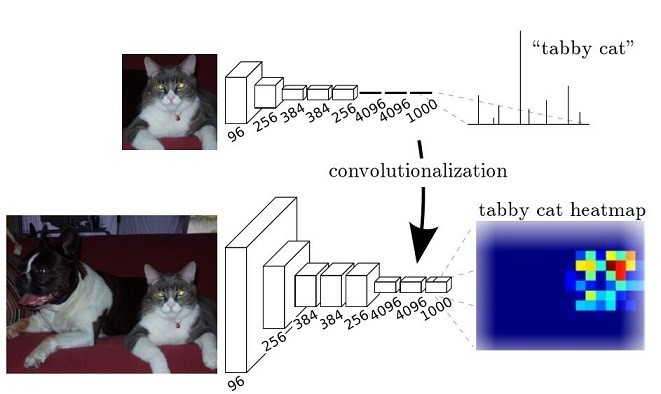
\includegraphics{./img/ch9/figure_9.1.1_2.jpg}
%\caption{}
\end{figure}

图 4

\subsection{9.3.2 FCN网络结构?}\label{fcnux7f51ux7edcux7ed3ux6784}

​ FCN对图像进行像素级的分类,从而解决了语义级别的图像分割(semantic
segmentation)问题。与经典的CNN在卷积层之后使用全连接层得到固定长度的特征向量进行分类(全联接层+softmax输出)不同,FCN可以接受任意尺寸的输入图像,采用反卷积层对最后一个卷积层的feature
map进行上采样,
使它恢复到输入图像相同的尺寸,从而可以对每个像素都产生了一个预测,
同时保留了原始输入图像中的空间信息,
最后在上采样的特征图上进行逐像素分类。 ​
下图是语义分割所采用的全卷积网络(FCN)的结构示意图:

\begin{figure}
\centering
%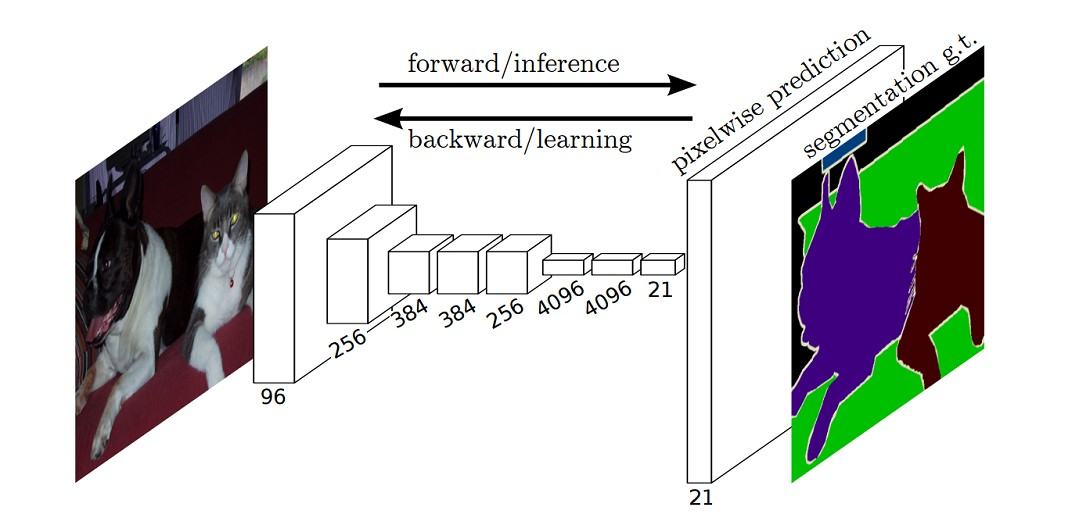
\includegraphics{./img/ch9/figure_9.1.2_1.jpg}
%\caption{}
\end{figure}

\subsection{9.3.3
全卷积网络举例?}\label{ux5168ux5377ux79efux7f51ux7edcux4e3eux4f8b}

​ 通常CNN网络在卷积层之后会接上若干个全连接层,
将卷积层产生的特征图(feature
map)映射成一个固定长度的特征向量。以AlexNet为代表的经典CNN结构适合于图像级的分类和回归任务,因为它们最后都得到整个输入图像的一个概率向量。

\begin{figure}
\centering
%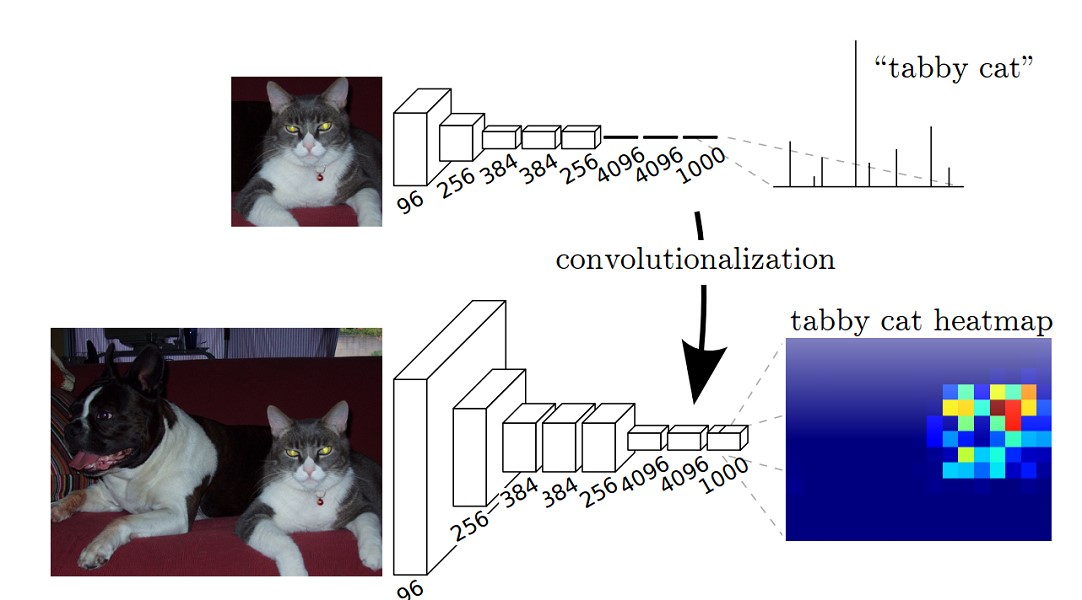
\includegraphics{./img/ch9/figure_9.1.3_1.jpg}
%\caption{}
\end{figure}

   如上图所示:\\
   (1)在CNN中, 猫的图片输入到AlexNet, 得到一个长为1000的输出向量,
表示输入图像属于每一类的概率, 其中在``tabby cat''这一类统计概率最高,
用来做分类任务。\\
  
(2)FCN与CNN的区别在于把CNN最后的全连接层转换成卷积层,输出的是一张已经带有标签的图片,
而这个图片就可以做语义分割。\\
  
(3)CNN的强大之处在于它的多层结构能自动学习特征,并且可以学习到多个层次的特征:
较浅的卷积层感知域较小,学习到一些局部区域的特征;较深的卷积层具有较大的感知域,能够学习到更加抽象一些的特征。高层的抽象特征对物体的大小、位置和方向等敏感性更低,从而有助于识别性能的提高,
所以我们常常可以将卷积层看作是特征提取器。

\subsection{9.2.4
全连接层和卷积层如何相互转化?}\label{ux5168ux8fdeux63a5ux5c42ux548cux5377ux79efux5c42ux5982ux4f55ux76f8ux4e92ux8f6cux5316}

   \textbf{两者相互转换的可能性:}\\
  
全连接层和卷积层之间唯一的不同就是卷积层中的神经元只与输入数据中的一个局部区域连接,并且在卷积列中的神经元共享参数。然而在两类层中,神经元都是计算点积,所以它们的函数形式是一样的。因此,将此两者相互转化是可能的:\\
  
(1)对于任一个卷积层,都存在一个能实现和它一样的前向传播函数的全连接层。权重矩阵是一个巨大的矩阵,除了某些特定块,其余部分都是零。而在其中大部分块中,元素都是相等的。\\
  
(2)任何全连接层都可以被转化为卷积层。比如VGG16中第一个全连接层是25088
* 4096的数据尺寸,将它转化为512 * 7 * 7 *
4096的数据尺寸,即一个K=4096的全连接层,输入数据体的尺寸是7 * 7 *
512,这个全连接层可以被等效地看做一个F=7, P=0, S=1, K=4096
的卷积层。换句话说,就是将滤波器的尺寸设置为和输入数据体的尺寸一致7 * 7,
这样输出就变为1 * 1 * 4096, 本质上和全连接层的输出是一样的。\\
   \textbf{输出激活数据体深度是由卷积核的数目决定的(K=4096)。}\\
  
在两种变换中,将全连接层转化为卷积层在实际运用中更加有用。假设一个卷积神经网络的输入是227x227x3的图像,一系列的卷积层和下采样层将图像数据变为尺寸为7x7x512的激活数据体,
AlexNet的处理方式为使用了两个尺寸为4096的全连接层,最后一个有1000个神经元的全连接层用于计算分类评分。我们可以将这3个全连接层中的任意一个转化为卷积层:\\
  
(1)第一个连接区域是{[}7x7x512{]}的全连接层,令其滤波器尺寸为F=7,K=4096,这样输出数据体就为{[}1x1x4096{]}。\\
  
(2)第二个全连接层,令其滤波器尺寸为F=1,K=4096,这样输出数据体为{[}1x1x4096{]}。\\
  
(3)最后一个全连接层也做类似的,令其F=1,K=1000,最终输出为{[}1x1x1000{]}。

\subsection{9.2.5
为什么传统CNN的输入图片是固定大小?}\label{ux4e3aux4ec0ux4e48ux4f20ux7edfcnnux7684ux8f93ux5165ux56feux7247ux662fux56faux5b9aux5927ux5c0f}

  
对于CNN,一幅输入图片在经过卷积和pooling层时,这些层是不关心图片大小的。比如对于一个卷积层,outputsize
= (inputsize - kernelsize) / stride +
1,它并不关心inputsize多大,对于一个inputsize大小的输入feature
map,滑窗卷积,输出outputsize大小的feature
map即可。pooling层同理。但是在进入全连接层时,feature
map(假设大小为n×n)要拉成一条向量,而向量中每个元素(共n×n个)作为一个结点都要与下一个层的所有结点(假设4096个)全连接,这里的权值个数是4096×n×n,而我们知道神经网络结构一旦确定,它的权值个数都是固定的,所以这个n不能变化,n是conv5的outputsize,所以层层向回看,每个outputsize都要固定,那每个inputsize都要固定,因此输入图片大小要固定。

\subsection{9.2.6
把全连接层的权重W重塑成卷积层的滤波器有什么好处?}\label{ux628aux5168ux8fdeux63a5ux5c42ux7684ux6743ux91cdwux91cdux5851ux6210ux5377ux79efux5c42ux7684ux6ee4ux6ce2ux5668ux6709ux4ec0ux4e48ux597dux5904}

   这样的转化可以在单个向前传播的过程中,
使得卷积网络在一张更大的输入图片上滑动,从而得到多个输出(可以理解为一个label
map)。\\
   比如:
我们想让224×224尺寸的浮窗,以步长为32在384×384的图片上滑动,把每个经停的位置都带入卷积网络,最后得到6×6个位置的类别得分,
那么通过将全连接层转化为卷积层之后的运算过程为:\\
  
如果224×224的输入图片经过卷积层和下采样层之后得到了{[}7x7x512{]}的数组,那么,384×384的大图片直接经过同样的卷积层和下采样层之后会得到{[}12x12x512{]}的数组,
然后再经过上面由3个全连接层转化得到的3个卷积层,最终得到{[}6x6x1000{]}的输出((12
-- 7)/1 + 1 = 6), 这个结果正是浮窗在原图经停的6×6个位置的得分。\\
  
一个确定的CNN网络结构之所以要固定输入图片大小,是因为全连接层权值数固定,而该权值数和feature
map大小有关,
但是FCN在CNN的基础上把1000个结点的全连接层改为含有1000个1×1卷积核的卷积层,经过这一层,还是得到二维的feature
map,同样我们也不关心这个feature map大小,
所以对于输入图片的size并没有限制。\\
  
如下图所示,FCN将传统CNN中的全连接层转化成卷积层,对应CNN网络FCN把最后三层全连接层转换成为三层卷积层:

\begin{figure}
\centering
%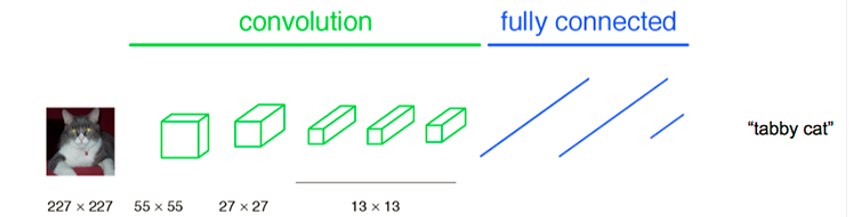
\includegraphics{./img/ch9/figure_9.1.7_1.png}
%\caption{}
\end{figure}

一个分类网络

\begin{figure}
\centering
%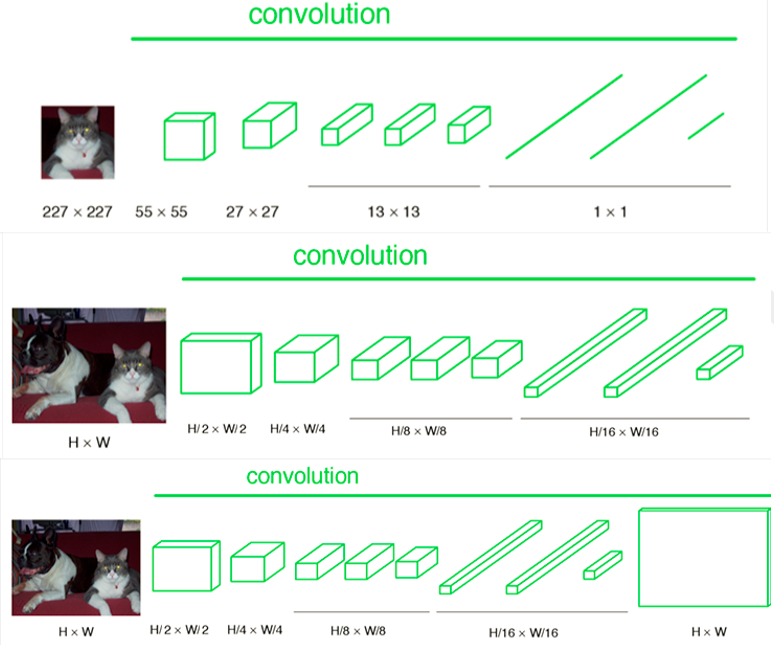
\includegraphics{./img/ch9/figure_9.1.7_2.png}
%\caption{}
\end{figure}

变为全卷积网络

\begin{figure}
\centering
%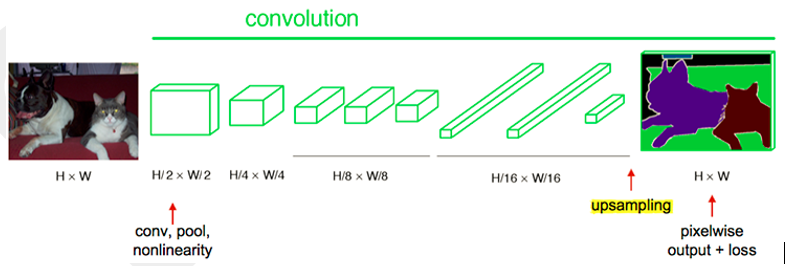
\includegraphics{./img/ch9/figure_9.1.7_3.png}
%\caption{}
\end{figure}

End-to-end, pixels-to pixels网络

\begin{figure}
\centering
%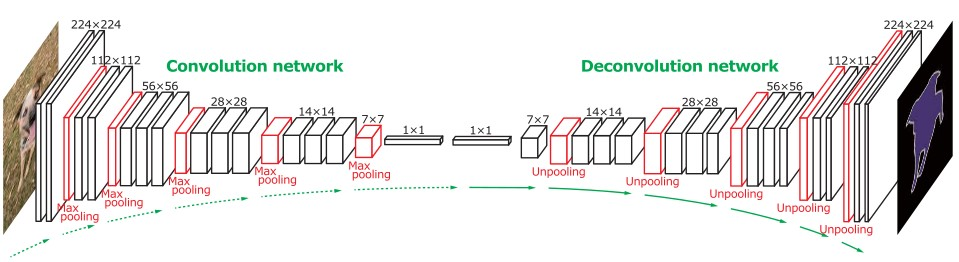
\includegraphics{./img/ch9/figure_9.1.7_4.jpg}
%\caption{}
\end{figure}

(1)全连接层转化为全卷积层 :
在传统的CNN结构中,前5层是卷积层,第6层和第7层分别是一个长度为4096的一维向量,第8层是长度为1000的一维向量,分别对应1000个不同类别的概率。FCN将这3层表示为卷积层,卷积核的大小
(通道数,宽,高) 分别为
(4096,1,1)、(4096,1,1)、(1000,1,1)。看上去数字上并没有什么差别,但是卷积跟全连接是不一样的概念和计算过程,使用的是之前CNN已经训练好的权值和偏置,但是不一样的在于权值和偏置是有自己的范围,属于自己的一个卷积核。\\
  
(2)CNN中输入的图像大小是统一固定成227x227大小的图像,第一层pooling后为55x55,第二层pooling后图像大小为27x27,第五层pooling后的图像大小为13x13,
而FCN输入的图像是H *
W大小,第一层pooling后变为原图大小的1/2,第二层变为原图大小的1/4,第五层变为原图大小的1/8,第八层变为原图大小的1/16。\\
  
(3)经过多次卷积和pooling以后,得到的图像越来越小,分辨率越来越低。其中图像到H/32
*
W/32的时候图片是最小的一层时,所产生图叫做heatmap热图,热图就是我们最重要的高维特征图,得到高维特征的heatmap之后就是最重要的一步也是最后的一步对原图像进行upsampling,把图像进行放大几次到原图像的大小。\\
  
相较于使用被转化前的原始卷积神经网络对所有36个位置进行迭代计算优化模型,然后再对36个位置做预测,使用转化后的卷积神经网络进行一次前向传播计算要高效得多,因为36次计算都在共享计算资源。这一技巧在实践中经常使用,通常将一张图像尺寸变得更大,然后使用变换后的卷积神经网络来对空间上很多不同位置进行评价得到分类评分,然后在求这些分值的平均值。

\subsection{9.2.7
反卷积层理解}\label{ux53cdux5377ux79efux5c42ux7406ux89e3}

  
Upsampling的操作可以看成是反卷积(deconvolutional),卷积运算的参数和CNN的参数一样是在训练FCN模型的过程中通过bp算法学习得到。反卷积层也是卷积层,不关心input大小,滑窗卷积后输出output。deconv并不是真正的deconvolution(卷积的逆变换),最近比较公认的叫法应该是transposed
convolution,deconv的前向传播就是conv的反向传播。\\
   反卷积参数:
利用卷积过程filter的转置(实际上就是水平和竖直方向上翻转filter)作为计算卷积前的特征图。\\
   反卷积的运算如下所示:\\
   蓝色是反卷积层的input,绿色是反卷积层的outputFull padding, transposed
Full padding, transposed。

\begin{figure}
\centering
%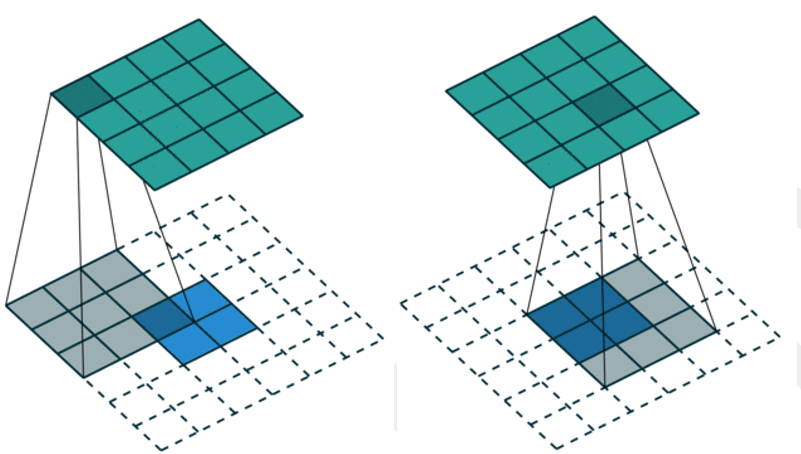
\includegraphics{./img/ch9/figure_9.1.8_1.png}
%\caption{}
\end{figure}

上图中的反卷积,input是2×2, output是4×4。 Zero padding, non-unit
strides, transposed。

%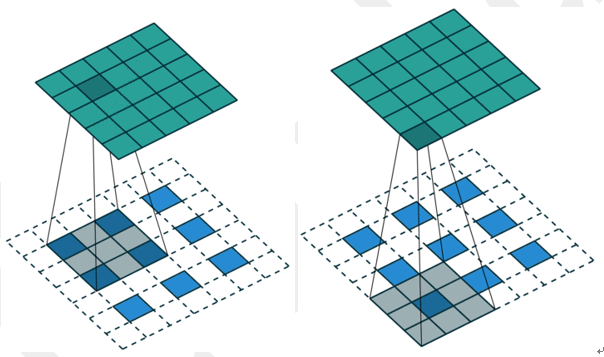
\includegraphics{./img/ch9/figure_9.1.8_2.png}

上图中的反卷积,input feature map是3×3, 转化后是5×5, output是5×5

\subsection{9.2.8 跳级(skip)结构}\label{ux8df3ux7ea7skipux7ed3ux6784}

   对CNN的结果做处理,得到了dense
prediction,而作者在试验中发现,得到的分割结果比较粗糙,所以考虑加入更多前层的细节信息,也就是把倒数第几层的输出和最后的输出做一个fusion,实际上也就是加和:

%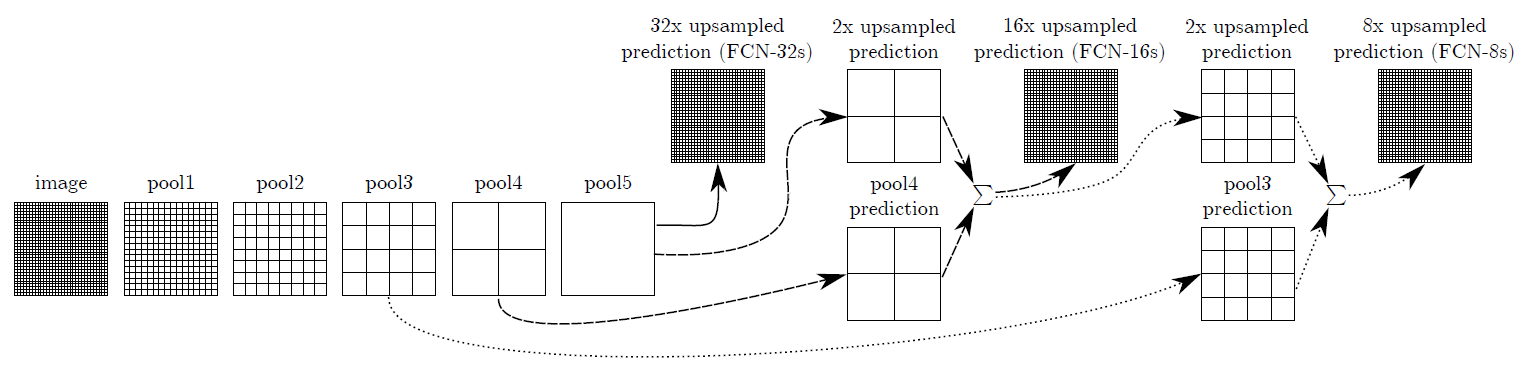
\includegraphics{./img/ch9/figure_9.1.9_1.png}\\
  
实验表明,这样的分割结果更细致更准确。在逐层fusion的过程中,做到第三行再往下,结果又会变差,所以作者做到这里就停了。

\subsection{9.2.9 模型训练}\label{ux6a21ux578bux8badux7ec3}

  
(1)用AlexNet,VGG16或者GoogleNet训练好的模型做初始化,在这个基础上做fine-tuning,全部都fine-tuning,只需在末尾加上upsampling,参数的学习还是利用CNN本身的反向传播原理。\\
   (2)采用whole image做训练,不进行patchwise
sampling。实验证明直接用全图已经很effective and efficient。\\
   (3)对class
score的卷积层做全零初始化。随机初始化在性能和收敛上没有优势。\\
\emph{举例:}\\
   \emph{FCN例子:
输入可为任意尺寸图像彩色图像;输出与输入尺寸相同,深度为:20类目标+背景=21,模型基于AlexNet。}\\
   \emph{蓝色:卷积层。}\\
   \emph{绿色:Max Pooling层。}\\
   \emph{黄色: 求和运算,
使用逐数据相加,把三个不同深度的预测结果进行融合:较浅的结果更为精细,较深的结果更为鲁棒。}\\
   \emph{灰色: 裁剪, 在融合之前,使用裁剪层统一两者大小,
最后裁剪成和输入相同尺寸输出。}\\
  
\emph{对于不同尺寸的输入图像,各层数据的尺寸(height,width)相应变化,深度(channel)不变。}

%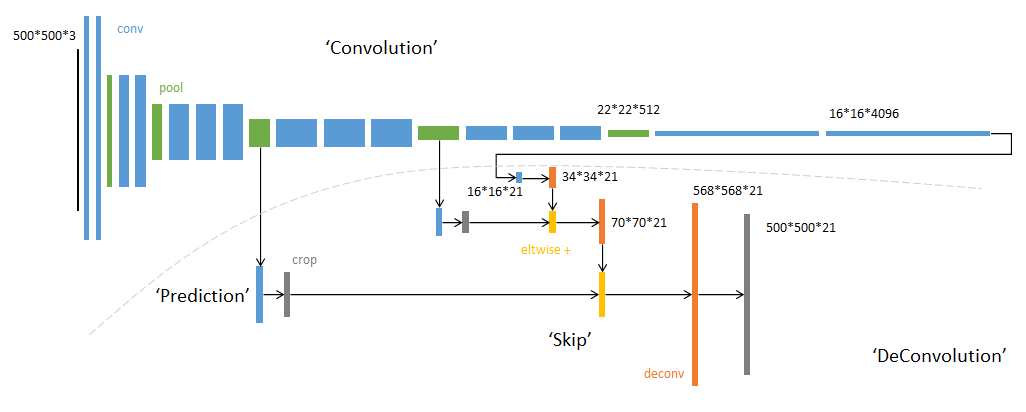
\includegraphics{./img/ch9/figure_9.1.10_1.png}\\
   (1)全卷积层部分进行特征提取,
提取卷积层(3个蓝色层)的输出来作为预测21个类别的特征。

   (2)图中虚线内是反卷积层的运算,
反卷积层(3个橙色层)可以把输入数据尺寸放大。和卷积层一样,升采样的具体参数经过训练确定。

     1)
以经典的AlexNet分类网络为初始化。最后两级是全连接(红色),参数弃去不用。

%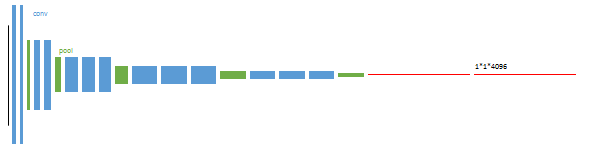
\includegraphics{./img/ch9/figure_9.1.10_2.png}      2)
从特征小图()预测分割小图(),之后直接升采样为大图。

\begin{figure}
\centering
%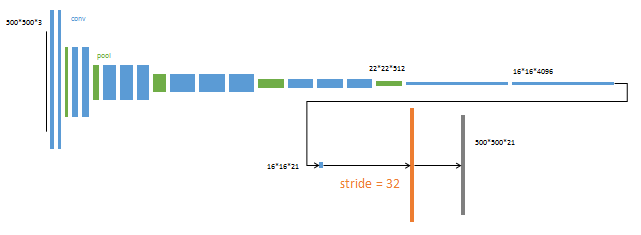
\includegraphics{./img/ch9/figure_9.1.10_3.png}
%\caption{}
\end{figure}

反卷积(橙色)的步长为32,这个网络称为FCN-32s

     3) 升采样分为两次完成(橙色×2),
在第二次升采样前,把第4个pooling层(绿色)的预测结果(蓝色)融合进来。使用跳级结构提升精确性。

\begin{figure}
\centering
%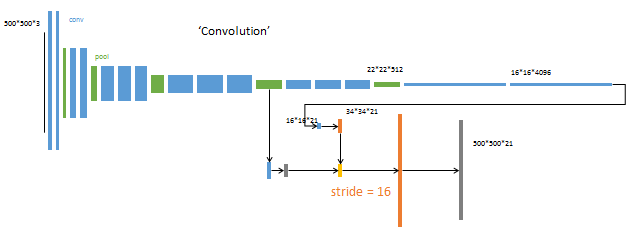
\includegraphics{./img/ch9/figure_9.1.10_4.png}
%\caption{}
\end{figure}

第二次反卷积步长为16,这个网络称为FCN-16s

     4) 升采样分为三次完成(橙色×3),
进一步融合了第3个pooling层的预测结果。

\begin{figure}
\centering
%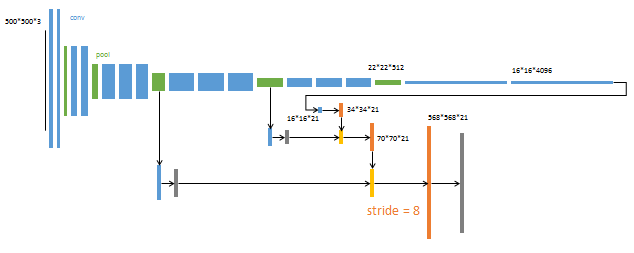
\includegraphics{./img/ch9/figure_9.1.10_5.png}
%\caption{}
\end{figure}

第三次反卷积步长为8,记为FCN-8s

其他参数:\\
   minibatch:20张图片。\\
   learning rate:0.001。\\
   初始化:分类网络之外的卷积层参数初始化为0。\\
   反卷积参数初始化为bilinear插值。\\
   最后一层反卷积固定位bilinear插值不做学习。

\begin{figure}
\centering
%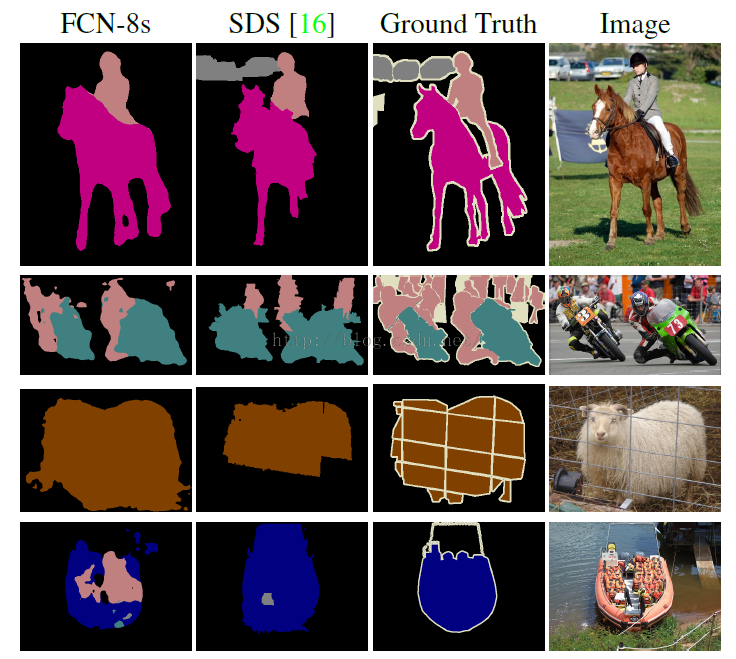
\includegraphics{./img/ch9/figure_9.1.10_6.png}
%\caption{}
\end{figure}

\subsection{9.2.10 FCN缺点}\label{fcnux7f3aux70b9}

  
(1)得到的结果还是不够精细。进行8倍上采样虽然比32倍的效果好了很多,但是上采样的结果还是比较模糊和平滑,对图像中的细节不敏感。\\
  
(2)对各个像素进行分类,没有充分考虑像素与像素之间的关系。忽略了在通常的基于像素分类的分割方法中使用的空间规整(spatial
regularization)步骤,缺乏空间一致性。

\section{9.3 U-Net}\label{u-net}

  
卷积网络被大规模应用在分类任务中,输出的结果是整个图像的类标签。然而,在许多视觉任务,尤其是生物医学图像处理领域,目标输出应该包括目标类别的位置,并且每个像素都应该有类标签。另外,在生物医学图像往往缺少训练图片。所以,Ciresan等人训练了一个卷积神经网络,用滑动窗口提供像素的周围区域(patch)作为输入来预测每个像素的类标签。这个网络有两个优点:
第一,输出结果可以定位出目标类别的位置;
第二,由于输入的训练数据是patches,这样就相当于进行了数据增广,解决了生物医学图像数量少的问题。\\
   但是,这个方法也有两个很明显缺点。\\
  
第一,它很慢,因为这个网络必须训练每个patch,并且因为patch间的重叠有很多的冗余(冗余会造成什么影响呢?卷积核里面的W,就是提取特征的权重,两个块如果重叠的部分太多,这个权重会被同一些特征训练两次,造成资源的浪费,减慢训练时间和效率,虽然说会有一些冗余,训练集大了,准确率不就高了吗?可是你这个是相同的图片啊,重叠的东西都是相同的,举个例子,我用一张相同的图片训练20次,按照这个意思也是增大了训练集啊,可是会出现什么结果呢,很显然,会导致过拟合,也就是对你这个图片识别很准,别的图片就不一定了)。\\
  
第二,定位准确性和获取上下文信息不可兼得。大的patches需要更多的max-pooling层这样减小了定位准确性(为什么?因为你是对以这个像素为中心的点进行分类,如果patch太大,最后经过全连接层的前一层大小肯定是不变的,如果你patch大就需要更多的pooling达到这个大小,而pooling层越多,丢失信息的信息也越多;小的patches只能看到很小的局部信息,包含的背景信息不够。\\
  
这篇论文建立了一个更好全卷积方法。我们定义和扩展了这个方法它使用更少的训练图片但产生更精确的分割。

\begin{figure}
\centering
%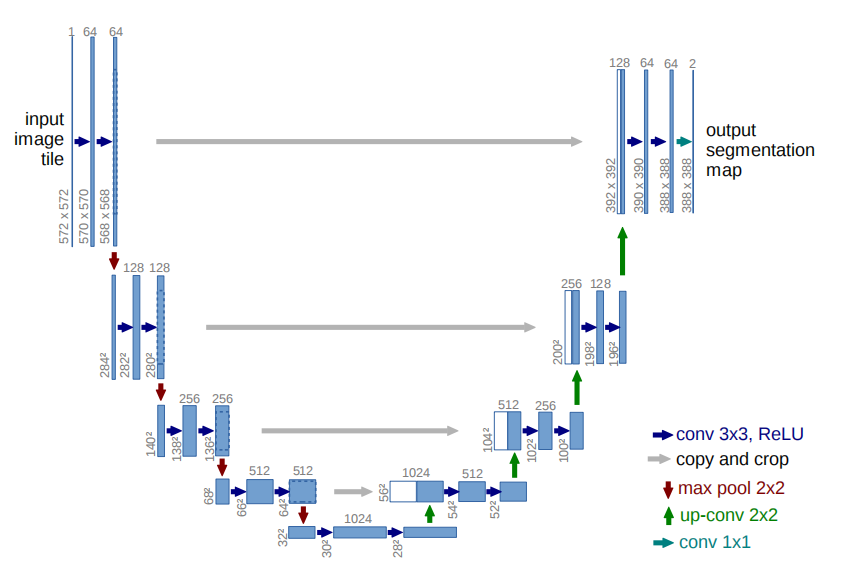
\includegraphics{./img/ch9/figure_9.2_1.png}
%\caption{}
\end{figure}

   (1)
使用全卷积神经网络。(全卷积神经网络就是卷积取代了全连接层,全连接层必须固定图像大小而卷积不用,所以这个策略使得,你可以输入任意尺寸的图片,而且输出也是图片,所以这是一个端到端的网络。)\\
   (2) 左边的网络是收缩路径:使用卷积和maxpooling。\\
   (3)
右边的网络是扩张路径:使用上采样产生的特征图与左侧收缩路径对应层产生的特征图进行concatenate操作。(pooling层会丢失图像信息和降低图像分辨率且是不可逆的操作,对图像分割任务有一些影响,对图像分类任务的影响不大,为什么要做上采样?因为上采样可以补足一些图片的信息,但是信息补充的肯定不完全,所以还需要与左边的分辨率比较高的图片相连接起来(直接复制过来再裁剪到与上采样图片一样大小),这就相当于在高分辨率和更抽象特征当中做一个折衷,因为随着卷积次数增多,提取的特征也更加有效,更加抽象,上采样的图片是经历多次卷积后的图片,肯定是比较高效和抽象的图片,然后把它与左边不怎么抽象但更高分辨率的特征图片进行连接)。\\
   (4)
最后再经过两次反卷积操作,生成特征图,再用两个1X1的卷积做分类得到最后的两张heatmap,例如第一张表示的是第一类的得分,第二张表示第二类的得分heatmap,然后作为softmax函数的输入,算出概率比较大的softmax类,选择它作为输入给交叉熵进行反向传播训练。

下面是U-Net模型的代码实现:(贡献者:黄钦建-华南理工大学)

\begin{verbatim}
def get_unet():
    inputs = Input((img_rows, img_cols, 1))
    conv1 = Conv2D(32, (3, 3), activation='relu', padding='same')(inputs)
    conv1 = Conv2D(32, (3, 3), activation='relu', padding='same')(conv1)
    pool1 = MaxPooling2D(pool_size=(2, 2))(conv1)
    # pool1 = Dropout(0.25)(pool1)
    # pool1 = BatchNormalization()(pool1)

    conv2 = Conv2D(64, (3, 3), activation='relu', padding='same')(pool1)
    conv2 = Conv2D(64, (3, 3), activation='relu', padding='same')(conv2)
    pool2 = MaxPooling2D(pool_size=(2, 2))(conv2)
    # pool2 = Dropout(0.5)(pool2)
    # pool2 = BatchNormalization()(pool2)

    conv3 = Conv2D(128, (3, 3), activation='relu', padding='same')(pool2)
    conv3 = Conv2D(128, (3, 3), activation='relu', padding='same')(conv3)
    pool3 = MaxPooling2D(pool_size=(2, 2))(conv3)
    # pool3 = Dropout(0.5)(pool3)
    # pool3 = BatchNormalization()(pool3)

    conv4 = Conv2D(256, (3, 3), activation='relu', padding='same')(pool3)
    conv4 = Conv2D(256, (3, 3), activation='relu', padding='same')(conv4)
    pool4 = MaxPooling2D(pool_size=(2, 2))(conv4)
    # pool4 = Dropout(0.5)(pool4)
    # pool4 = BatchNormalization()(pool4)

    conv5 = Conv2D(512, (3, 3), activation='relu', padding='same')(pool4)
    conv5 = Conv2D(512, (3, 3), activation='relu', padding='same')(conv5)

    up6 = concatenate([Conv2DTranspose(256, (2, 2), strides=(
        2, 2), padding='same')(conv5), conv4], axis=3)
    # up6 = Dropout(0.5)(up6)
    # up6 = BatchNormalization()(up6)
    conv6 = Conv2D(256, (3, 3), activation='relu', padding='same')(up6)
    conv6 = Conv2D(256, (3, 3), activation='relu', padding='same')(conv6)

    up7 = concatenate([Conv2DTranspose(128, (2, 2), strides=(
        2, 2), padding='same')(conv6), conv3], axis=3)
    # up7 = Dropout(0.5)(up7)
    # up7 = BatchNormalization()(up7)
    conv7 = Conv2D(128, (3, 3), activation='relu', padding='same')(up7)
    conv7 = Conv2D(128, (3, 3), activation='relu', padding='same')(conv7)

    up8 = concatenate([Conv2DTranspose(64, (2, 2), strides=(
        2, 2), padding='same')(conv7), conv2], axis=3)
    # up8 = Dropout(0.5)(up8)
    # up8 = BatchNormalization()(up8)
    conv8 = Conv2D(64, (3, 3), activation='relu', padding='same')(up8)
    conv8 = Conv2D(64, (3, 3), activation='relu', padding='same')(conv8)

    up9 = concatenate([Conv2DTranspose(32, (2, 2), strides=(
        2, 2), padding='same')(conv8), conv1], axis=3)
    # up9 = Dropout(0.5)(up9)
    # up9 = BatchNormalization()(up9)
    conv9 = Conv2D(32, (3, 3), activation='relu', padding='same')(up9)
    conv9 = Conv2D(32, (3, 3), activation='relu', padding='same')(conv9)

    # conv9 = Dropout(0.5)(conv9)

    conv10 = Conv2D(1, (1, 1), activation='sigmoid')(conv9)

    model = Model(inputs=[inputs], outputs=[conv10])

    model.compile(optimizer=Adam(lr=1e-5),
                  loss=dice_coef_loss, metrics=[dice_coef])

    return model
\end{verbatim}

\section{9.4 SegNet}\label{segnet}

  
可训练的图像分割引擎,包含一个encoder网络,一个对应的decoder网络,衔接像素级分类层,解码网络与VGG16的13层卷积层相同。解码网络是将低分辨率的编码特征图映射到全分辨率的特征图。解码网络使用最大池化层的池化索引进行非线性上采样,上采样过程就不需要学习。上采样得到的稀疏图与可训练的滤波器卷积得到致密的特征图。\\
   使用池化层索引进行上采样的优势:\\
   1)提升边缘刻画度;\\
   2)减少训练的参数;\\
   3)这种上采样模式可以包含到任何编码-解码网络中。\\
   SegNet网络的结构如下图所示:

\begin{figure}
\centering
%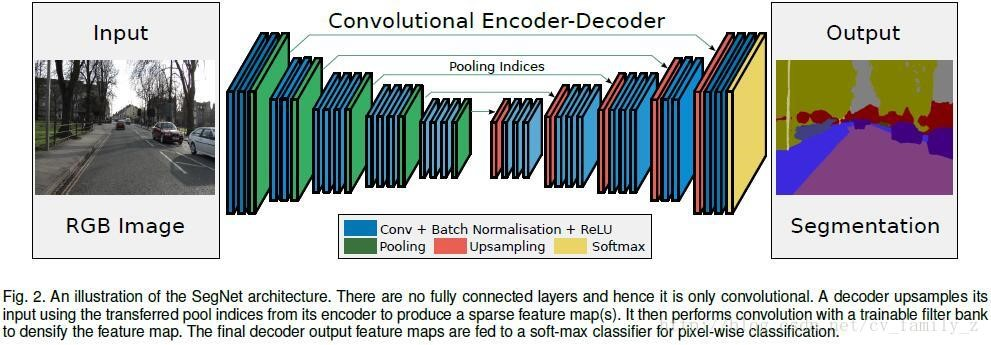
\includegraphics{./img/ch9/figure_9.3_1.jpg}
%\caption{}
\end{figure}

  
SegNet网络结构如图1所示,Input为输入图片,Output为输出分割的图像,不同颜色代表不同的分类。语义分割的重要性就在于不仅告诉你图片中某个东西是什么,而且告知你他在图片的位置。我们可以看到是一个对称网络,由中间绿色pooling层与红色upsampling层作为分割,左边是卷积提取高维特征,并通过pooling使图片变小,SegNet作者称为Encoder,右边是反卷积(在这里反卷积与卷积没有区别)与upsampling,通过反卷积使得图像分类后特征得以重现,upsampling使图像变大,SegNet作者称为Decoder,最后通过Softmax,输出不同分类的最大值。这就是大致的SegNet过程,下面对这个过程里面使用到的方法进行介绍。\\
  
编码网络与滤波器族卷积得到特征图,进行BN,ReLU,最大池化。最大池化是为了获得空间小位移的平移不变。最大池化和下采样损失了边缘细节,因此,在编码过程中保存边缘信息很重要。考虑到内存原因,只保存最大池化索引,如最大特征值的位置。\\
   SegNet解码技术如下图所示:

\begin{figure}
\centering
%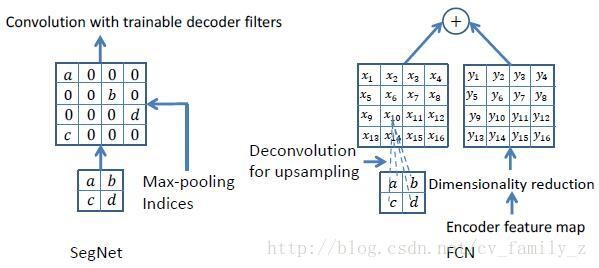
\includegraphics{./img/ch9/figure_9.3_2.jpg}
%\caption{}
\end{figure}

  
解码网络使用保存的最大池化索引上采样,得到稀疏的特征图,将特征图与可训练的解码滤波器族卷积得到致密的特征图。之后进行BN。高维的特征图输入soft-max层,对每个像素进行分类,得到每个像素属于K类的概率。
图3中右边是FCN的解码技术,FCN对编码的特征图进行降维,降维后输入到解码网络,解码网络中,上采样使用反卷积实现,上采样的特征图与降维的编码图进行element-wise
add得到最终的解码特征图。FCN解码模型需要存储编码特征图,在嵌入式设备中内存紧张。\\
  
SegNet的Encoder过程中,卷积的作用是提取特征,SegNet使用的卷积为same卷积(详见卷积神经网络CNN(1)),即卷积后不改变图片大小;在Decoder过程中,同样使用same卷积,不过卷积的作用是为upsampling变大的图像丰富信息,使得在Pooling过程丢失的信息可以通过学习在Decoder得到。SegNet中的卷积与传统CNN的卷积并没有区别。

\section{9.5 空洞卷积(Dilated
Convolutions)}\label{ux7a7aux6d1eux5377ux79efdilated-convolutions}

  
在图像分割领域,图像输入到CNN(典型的网络比如FCN{[}3{]})中,FCN先像传统的CNN那样对图像做卷积再pooling,降低图像尺寸的同时增大感受野,但是由于图像分割预测是pixel-wise的输出,所以要将pooling后较小的图像尺寸upsampling到原始的图像尺寸进行预测(upsampling一般采用deconv反卷积操作,deconv可参见知乎答案如何理解深度学习中的deconvolution
networks?),之前的pooling操作使得每个pixel预测都能看到较大感受野信息。因此图像分割FCN中有两个关键,一个是pooling减小图像尺寸增大感受野,另一个是upsampling扩大图像尺寸。在先减小再增大尺寸的过程中,肯定有一些信息损失掉了,那么能不能设计一种新的操作,不通过pooling也能有较大的感受野看到更多的信息呢?答案就是dilated
conv。\\
   以前的CNN主要问题总结:\\
   (1)Up-sampling / pooling layer\\
   (2)内部数据结构丢失;空间层级化信息丢失。\\
   (3)小物体信息无法重建 (假设有四个pooling layer 则 任何小于 2\^{}4 =
16 pixel 的物体信息将理论上无法重建。)\\
   举例如下:

\begin{figure}
\centering
%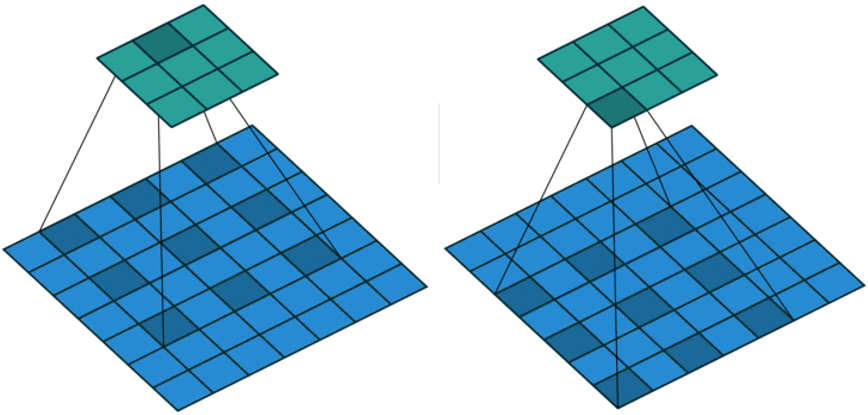
\includegraphics{./img/ch9/figure_9.3_3.png}
%\caption{}
\end{figure}

Dilated Convolution with a 3 x 3 kernel and dilation rate 2

   下面看一下dilated conv原始论文{[}4{]}中的示意图

\begin{figure}
\centering
%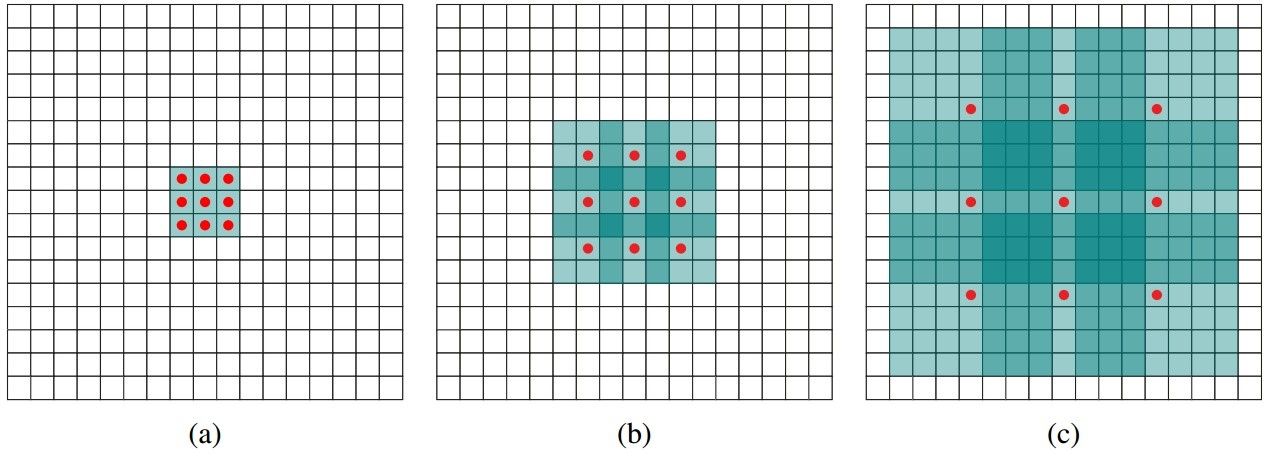
\includegraphics{./img/ch9/figure_9.3_4.jpg}
%\caption{}
\end{figure}

   (a) 图对应3x3的1-dilated
conv,和普通的卷积操作一样,(b)图对应3x3的2-dilated
conv,实际的卷积kernel
size还是3x3,但是空洞为1,也就是对于一个7x7的图像patch,只有9个红色的点和3x3的kernel发生卷积操作,其余的点略过。也可以理解为kernel的size为7x7,但是只有图中的9个点的权重不为0,其余都为0。
可以看到虽然kernel
size只有3x3,但是这个卷积的感受野已经增大到了7x7(如果考虑到这个2-dilated
conv的前一层是一个1-dilated
conv的话,那么每个红点就是1-dilated的卷积输出,所以感受野为3x3,所以1-dilated和2-dilated合起来就能达到7x7的conv),(c)图是4-dilated
conv操作,同理跟在两个1-dilated和2-dilated
conv的后面,能达到15x15的感受野。对比传统的conv操作,3层3x3的卷积加起来,stride为1的话,只能达到(kernel-1)
* layer+1=7的感受野,也就是和层数layer成线性关系,而dilated
conv的感受野是指数级的增长。\\
  
dilated的好处是不做pooling损失信息的情况下,加大了感受野,让每个卷积输出都包含较大范围的信息。在图像需要全局信息或者语音文本需要较长的sequence信息依赖的问题中,都能很好的应用dilated
conv,比如图像分割、语音合成WaveNet、机器翻译ByteNet中。

\section{9.6 RefineNet}\label{refinenet}

   网络结构:\\
   RefineNet block的作用就是把不同resolution level的feature
map进行融合。网络结构如下:

%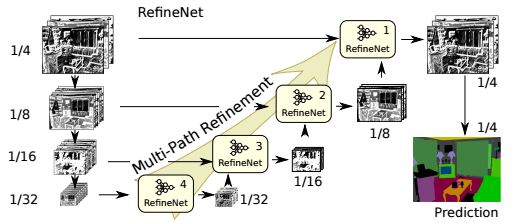
\includegraphics{./img/ch9/figure_9.4_1.png}\\
   最左边一栏就是FCN的encoder部分(文中是用的ResNet),先把pretrained
ResNet按feature map的分辨率分成四个ResNet
blocks,然后向右把四个blocks分别作为4个path通过RefineNet
block进行融合refine,最后得到一个refined feature
map(接softmax再双线性插值输出)。 注意除了RefineNet-4,所有的RefineNet
block都是二输入的,用于融合不同level做refine,而单输入的RefineNet-4可以看作是先对ResNet的一个task
adaptation。

   \textbf{RefineNet Block}\\
   接下来仔细看一下RefineNet block,可以看到主要组成部分是Residual
convolution unit, Multi-resolution fusion, Chained residual pooling,
Output convolutions. 切记这个block作用是融合多个level的feature
map输出单个level的feature
map,但具体的实现应该是和输入个数、shape无关的。

\begin{figure}
\centering
%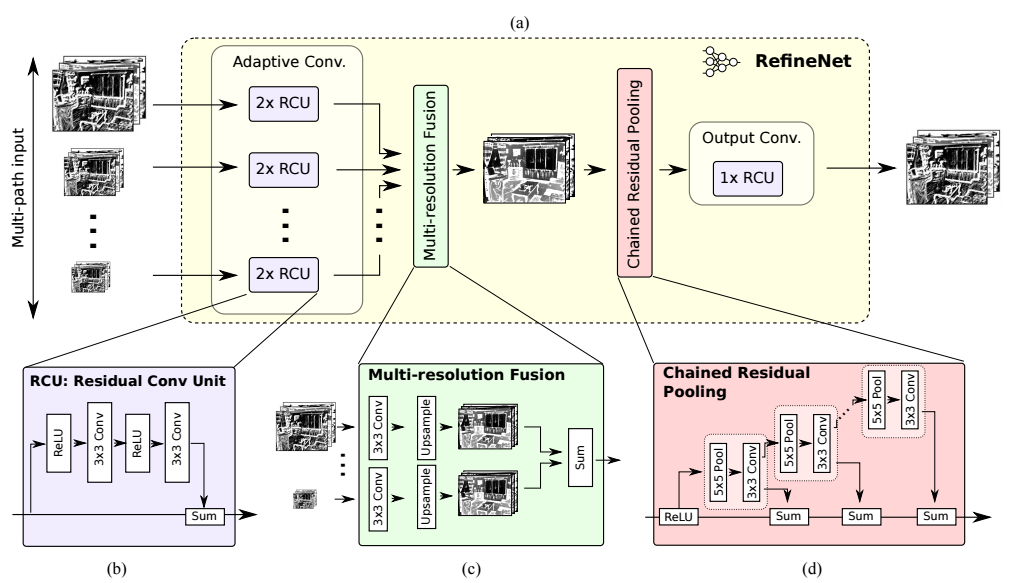
\includegraphics{./img/ch9/figure_9.4_2.png}
%\caption{}
\end{figure}

   Residual convolution unit就是普通的去除了BN的residual unit;

   Multi-resolution fusion是先对多输入的feature
map都用一个卷积层进行adaptation(都化到最小的feature
map的shape),再上采样再做element-wise的相加。注意如果是像RefineNet-4那样的单输入block这一部分就直接pass了;

   Chained residual
pooling中的ReLU对接下来池化的有效性很重要,还可以使模型对学习率的变化没这么敏感。这个链式结构能从很大范围区域上获取背景context。另外,这个结构中大量使用了identity
mapping这样的连接,无论长距离或者短距离的,这样的结构允许梯度从一个block直接向其他任一block传播。

   Output convolutions就是输出前再加一个RCU。

\section{9.7 PSPNet}\label{pspnet}

  
场景解析对于无限制的开放词汇和不同场景来说是具有挑战性的.本文使用文中的pyramid
pooling
module实现基于不同区域的上下文集成,提出了PSPNet,实现利用上下文信息的能力进行场景解析。\\
  
作者认为,FCN存在的主要问题是没有采取合适的策略来用全局的信息,本文的做法就是借鉴SPPNet来设计了PSPNet解决这个问题。\\
  
很多State-of-the-art的场景解析框架都是基于FCN的.基于CNN的方法能够增强动态物体的理解,但是在无限制词汇和不同场景中仍然面临挑战.举个例子,如下图.

%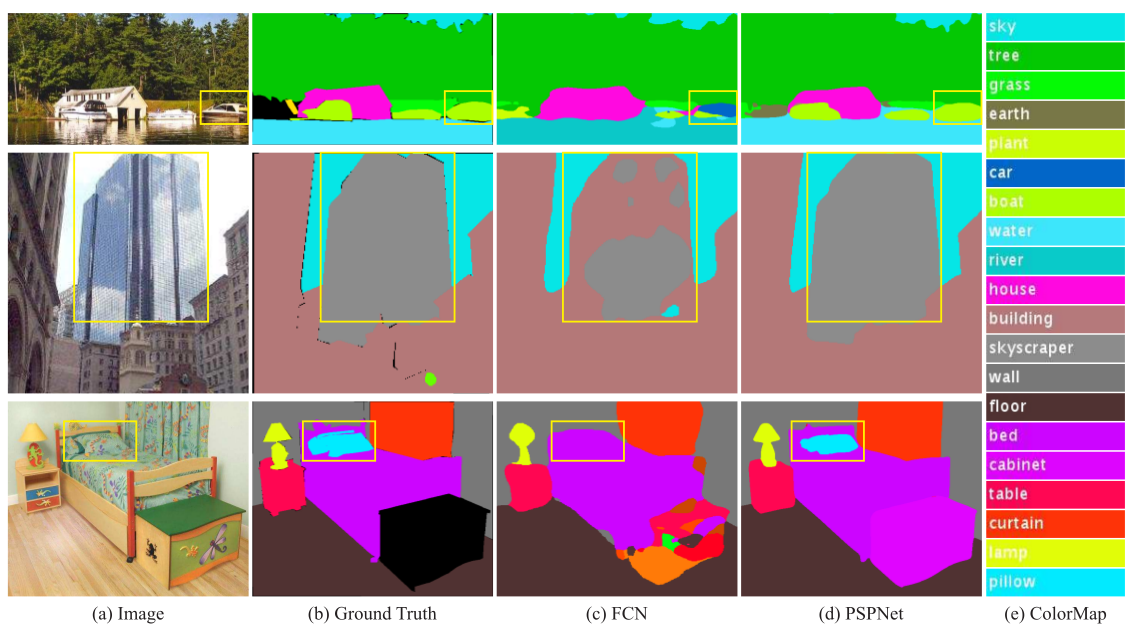
\includegraphics{./img/ch9/figure_9.6_1.png}\\
  
FCN认为右侧框中是汽车,但是实际上是船,如果参考上下文的先验知识,就会发现左边是一个船屋,进而推断是框中是船.FCN存在的主要问题就是不能利用好全局的场景线索。

  
对于尤其复杂的场景理解,之前都是采用空间金字塔池化来做的,和之前方法不同(为什么不同,需要参考一下经典的金字塔算法),本文提出了pyramid
scene parsing network(PSPNet)。\\
   本文的主要贡献如下:\\
   (1) 提出了PSPNet在基于FCN的框架中集成困难的上下文特征\\
   (2) 通过基于深度监督误差开发了针对ResNet的高效优化策略\\
   (3)
构建了一个用于state-of-the-art的场景解析和语义分割的实践系统(具体是什么?)\\
   通过观察FCN的结果,发现了如下问题:\\
   (1) 关系不匹配(Mismatched Relationship)\\
   (2) 易混淆的类别(Confusion Categories)\\
   (3) 不显眼的类别(Inconspicuous Classes)\\
  
总结以上结果发现,以上问题部分或者全部与上下文关系和全局信息有关系,因此本文提出了PSPNet.框架如下:

%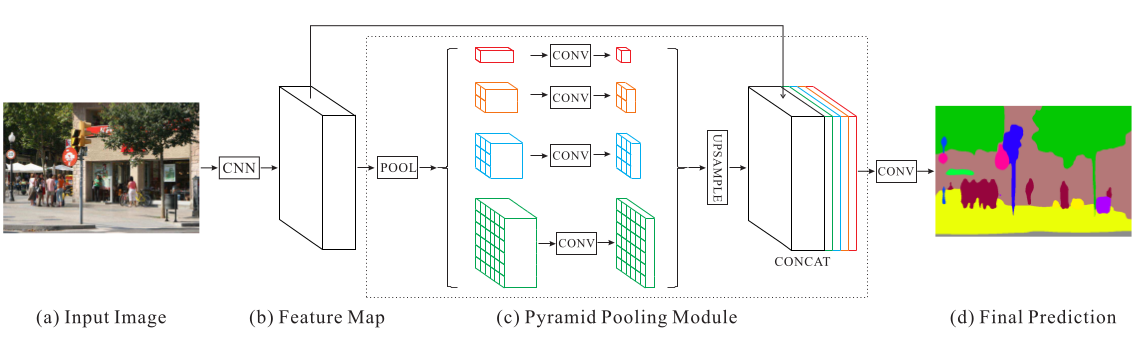
\includegraphics{./img/ch9/figure_9.6_2.png}\\
   并且加入额外的深度监督 Loss

\begin{figure}
\centering
%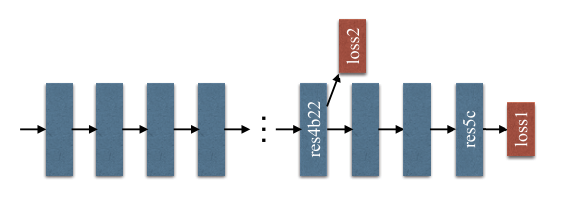
\includegraphics{./img/ch9/figure_9.6_3.png}
%\caption{}
\end{figure}

\section{9.8 DeepLab系列}\label{deeplabux7cfbux5217}

\subsection{9.8.1 DeepLabv1}\label{deeplabv1}

   DeepLab
是结合了深度卷积神经网络(DCNNs)和概率图模型(DenseCRFs)的方法。\\
   在实验中发现 DCNNs 做语义分割时精准度不够的问题,根本原因是 DCNNs
的高级特征的平移不变性,即高层次特征映射,根源于重复的池化和下采样。\\
   针对信号下采样或池化降低分辨率,DeepLab 是采用的
atrous(带孔)算法扩展感受野,获取更多的上下文信息。\\
   分类器获取以对象中心的决策是需要空间变换的不变性,这天然地限制了 DCNN
的定位精度,DeepLab
采用完全连接的条件随机场(CRF)提高模型捕获细节的能力。\\
   除空洞卷积和 CRFs 之外,论文使用的 tricks 还有 Multi-Scale
features。其实就是 U-Net 和 FPN
的思想,在输入图像和前四个最大池化层的输出上附加了两层的 MLP,第一层是
128 个 3×3 卷积,第二层是 128 个 1×1
卷积。最终输出的特征与主干网的最后一层特征图融合,特征图增加 5×128=640
个通道。\\
   实验表示多尺度有助于提升预测结果,但是效果不如 CRF 明显。\\
   论文模型基于 VGG16,在 Titan GPU 上运行速度达到了 8FPS,全连接 CRF
平均推断需要 0.5s ,在 PASCAL VOC-2012 达到 71.6\% IOU accuracy。

\subsection{9.8.2 DeepLabv2}\label{deeplabv2}

   DeepLabv2 是相对于 DeepLabv1 基础上的优化。DeepLabv1
在三个方向努力解决,但是问题依然存在:特征分辨率的降低、物体存在多尺度,DCNN
的平移不变性。\\
   因 DCNN 连续池化和下采样造成分辨率降低,DeepLabv2
在最后几个最大池化层中去除下采样,取而代之的是使用空洞卷积,以更高的采样密度计算特征映射。\\
   物体存在多尺度的问题,DeepLabv1 中是用多个 MLP
结合多尺度特征解决,虽然可以提供系统的性能,但是增加特征计算量和存储空间。\\
   论文受到 Spatial Pyramid Pooling (SPP)
的启发,提出了一个类似的结构,在给定的输入上以不同采样率的空洞卷积并行采样,相当于以多个比例捕捉图像的上下文,称为
ASPP (atrous spatial pyramid pooling) 模块。\\
   DCNN 的分类不变形影响空间精度。DeepLabv2 是采样全连接的 CRF
在增强模型捕捉细节的能力。\\
   论文模型基于 ResNet,在 NVidia Titan X GPU 上运行速度达到了
8FPS,全连接 CRF 平均推断需要 0.5s ,在耗时方面和 DeepLabv1 无差异,但在
PASCAL VOC-2012 达到 79.7 mIOU。

\subsection{9.8.3 DeepLabv3}\label{deeplabv3}

   好的论文不止说明怎么做,还告诉为什么。DeepLab 延续到 DeepLabv3
系列,依然是在空洞卷积做文章,但是探讨不同结构的方向。\\
   DeepLabv3 论文比较了多种捕获多尺度信息的方式:

\begin{figure}
\centering
%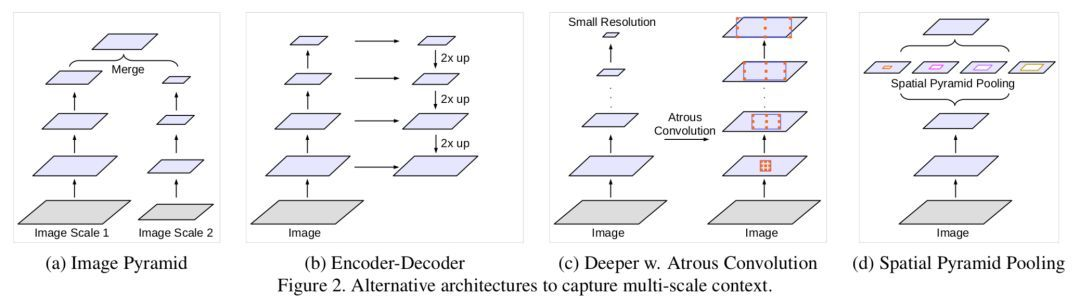
\includegraphics{./img/ch9/figure_9.6_4.png}
%\caption{}
\end{figure}

   1.Image Pyramid:将输入图片放缩成不同比例,分别应用在 DCNN
上,将预测结果融合得到最终输出。\\
   2.Encoder-Decoder:利用 Encoder 阶段的多尺度特征,运用到 Decoder
阶段上恢复空间分辨率,代表工作有 FCN、SegNet、PSPNet 等工。\\
   3.Deeper w. Atrous Convolution:在原始模型的顶端增加额外的模块,例如
DenseCRF,捕捉像素间长距离信息。\\
   4.Spatial Pyramid
Pooling:空间金字塔池化具有不同采样率和多种视野的卷积核,能够以多尺度捕捉对象。\\
   DeepLabv1-v2
都是使用带孔卷积提取密集特征来进行语义分割。但是为了解决分割对象的多尺度问题,DeepLabv3
设计采用多比例的带孔卷积级联或并行来捕获多尺度背景。\\
   此外,DeepLabv3
将修改之前提出的带孔空间金字塔池化模块,该模块用于探索多尺度卷积特征,将全局背景基于图像层次进行编码获得特征,取得
state-of-art 性能,在 PASCAL VOC-2012 达到 86.9 mIOU。

\subsection{9.8.4 DeepLabv3+}\label{deeplabv3-1}

   语义分割关注的问题:\\
   1、 实例对象多尺度问题。\\
   2、
因为深度网络存在stride=2的层,会导致feature分辨率下降,从而导致预测精度降低,而造成的边界信息丢失问题。\\
   deeplab V3新设计的aspp结构解决了问题1,deeplab
v3+主要目的在于解决问题2。\\
   问题2
可以使用空洞卷积替代更多的pooling层来获取分辨率更高的feature。但是feature分辨率更高会极大增加运算量。以deeplab
v3使用的resnet101为例,stride=16将造成后面9层feature变大,后面9层的计算量变为原来的2*2=4倍大。stride=8则更为恐怖,后面78层的计算量都会变大很多。\\
   解决方案:1、编解码器结构;2 Modified Aligned Xception

\begin{figure}
\centering
%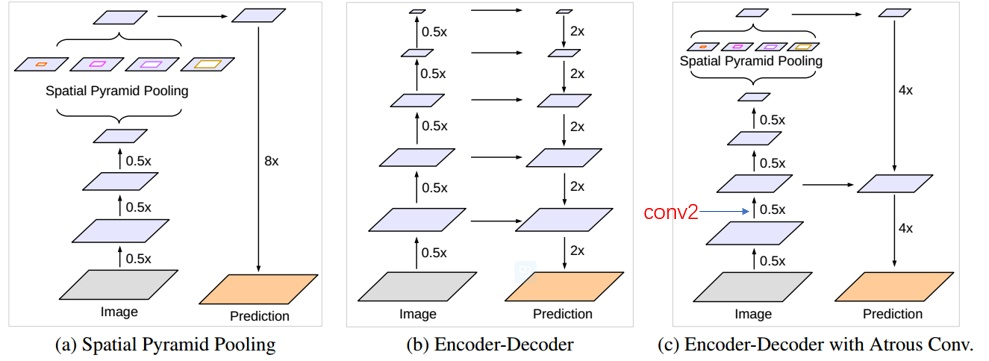
\includegraphics{./img/ch9/figure_9.6_5.png}
%\caption{}
\end{figure}

  
在deeplabv3基础上加入解码器。A是aspp结构,其中8x的上采样可以看做是一个解码器。B是编解码结构,它集合了高层和底层的特征。C就是本文采取的结构。
   方法:\\
   (1)Encoder-Decoder with Atrous Convolution

\begin{figure}
\centering
%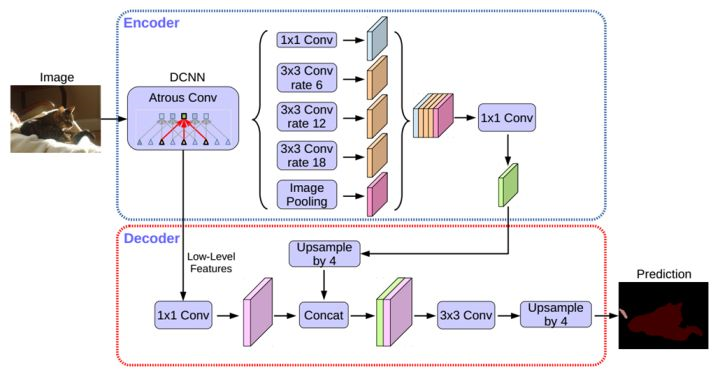
\includegraphics{./img/ch9/figure_9.6_6.png}
%\caption{}
\end{figure}

   编码器采用deeplabv3。\\
   解码器部分:先从低层级选一个feature,将低层级的feature用1 *
1的卷积进行通道压缩(原本为256通道,或者512通道),目的在于减少低层级的比重。作者认为编码器得到的feature具有更丰富的信息,所以编码器的feature应该有更高的比重。
这样做有利于训练。\\
  
再将编码器的输出上采样,使其分辨率与低层级feature一致。举个例子,如果采用resnet
conv2 输出的feature,则这里要* 4上采样。将两种feature连接后,再进行一次3
*
3的卷积(细化作用),然后再次上采样就得到了像素级的预测。后面的实验结果表明这种结构在
stride=16
时既有很高的精度速度又很快。stride=8相对来说只获得了一点点精度的提升,但增加了很多的计算量。\\
   (2)Modified Aligned Xception\\
   Xception主要采用了deepwish seperable
convolution来替换原来的卷积层。简单的说就是这种结构能在更少参数更少计算量的情况下学到同样的信息。这边则是考虑将原来的resnet-101骨架网换成xception。

\begin{figure}
\centering
%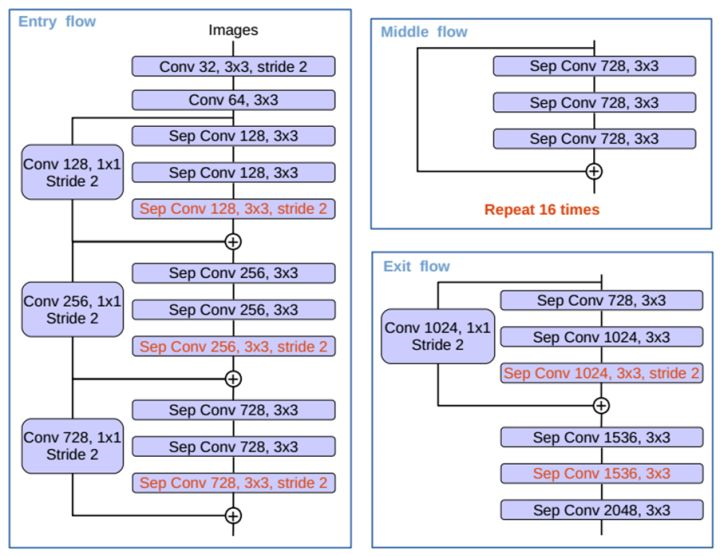
\includegraphics{./img/ch9/figure_9.6_7.png}
%\caption{}
\end{figure}

   \textbf{红色部分为修改}\\
   更多层:重复8次改为16次(基于MSRA目标检测的工作)。\\
   将原来简单的pool层改成了stride为2的deepwish seperable convolution。\\
   额外的RELU层和归一化操作添加在每个 3 × 3 depthwise
convolution之后(原来只在1 * 1卷积之后)

\section{9.9 Mask-R-CNN}\label{mask-r-cnn}

\subsection{9.9.1 Mask-RCNN
的网络结构示意图}\label{mask-rcnn-ux7684ux7f51ux7edcux7ed3ux6784ux793aux610fux56fe}

\begin{figure}
\centering
%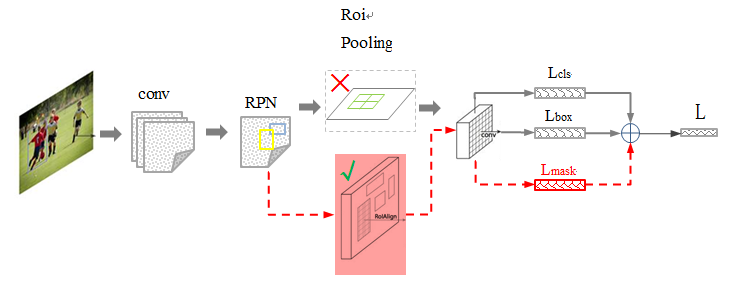
\includegraphics{./img/ch9/figure_9.8_1.png}
%\caption{}
\end{figure}

   其中黑色部分为原来的Faster-RCNN,红色部分为在Faster网络上的修改:\\
   1)将ROI Pooling层替换成了ROIAlign;\\
   2)添加并列的FCN层(Mask层);\\
  
先来概述一下Mask-RCNN的几个特点(来自于Paper\href{https://arxiv.org/pdf/1703.06870.pdf}{Mask
R-CNN}的Abstract):\\
   1)在边框识别的基础上添加分支网络,用于语义Mask识别;\\
   2)训练简单,相对于Faster仅增加一个小的Overhead,可以跑到5FPS;\\
   3)可以方便的扩展到其他任务,比如人的姿态估计等;\\
   4)不借助Trick,在每个任务上,效果优于目前所有的 single-model
entries;包括 COCO 2016 的Winners。

\subsection{9.9.2
RCNN行人检测框架}\label{rcnnux884cux4ebaux68c0ux6d4bux6846ux67b6}

   来看下后面两种RCNN方法与Mask结合的示意图:

%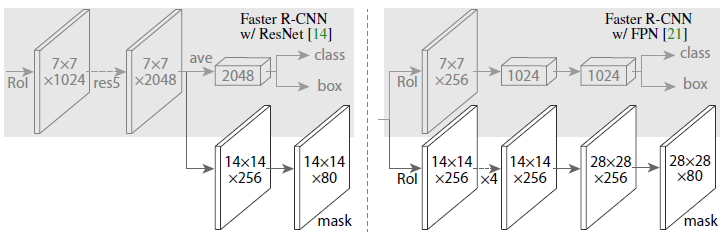
\includegraphics{./img/ch9/figure_9.8_2.png}\\
   图中灰色部分是原来的RCNN结合ResNet or
FPN的网络,下面黑色部分为新添加的并联Mask层,这个图本身与上面的图也没有什么区别,旨在说明作者所提出的Mask
RCNN方法的泛化适应能力:可以和多种RCNN框架结合,表现都不错。

\subsection{9.9.3 Mask-RCNN
技术要点}\label{mask-rcnn-ux6280ux672fux8981ux70b9}

   \textbf{1.技术要点1 - 强化的基础网络}\\
   通过ResNeXt-101+FPN用作特征提取网络,达到state-of-the-art的效果。\\
   \textbf{2.技术要点2 - ROIAlign}\\
  
采用ROIAlign替代RoiPooling(改进池化操作)。引入了一个插值过程,先通过双线性插值到14\emph{14,再pooling到7}7,很大程度上解决了仅通过Pooling直接采样带来的Misalignment对齐问题。\\
   PS: 虽然 Misalignment 在分类问题上影响并不大,但在 Pixel 级别的 Mask
上会存在较大误差。\\
   后面我们把结果对比贴出来(Table2 c \& d),能够看到 ROIAlign
带来较大的改进,可以看到,Stride 越大改进越明显。\\
   \textbf{3.技术要点3 - Loss Function}\\
   每个ROIAlign对应K *
m\^{}2维度的输出。K对应类别个数,即输出K个mask,m对应池化分辨率(7 *
7)。Loss函数定义: \[
Lmask(Cls_k)=Sigmoid(Cls_k)
\]    \(Lmask(Cls_k) = Sigmoid (Cls_k)\),平均二值交叉熵 (average
binary cross-entropy)Loss,通过逐像素的 Sigmoid 计算得到。\\
   Why K个mask?通过对每个 Class
对应一个Mask可以有效避免类间竞争(其他Class不贡献Loss)。

%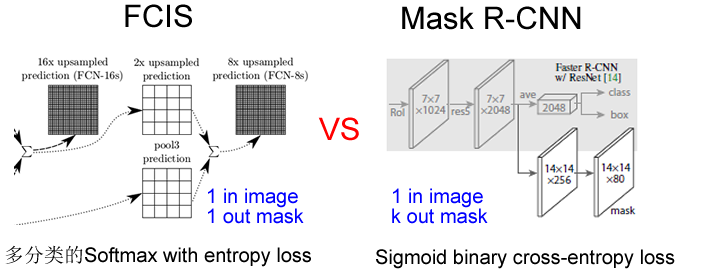
\includegraphics{./img/ch9/figure_9.8_3.png}\\
   通过结果对比来看(Table2 b),也就是作者所说的 Decouple
解耦,要比多分类的Softmax效果好很多。\\
  
另外,作者给出了很多实验分割效果,就不都列了,只贴一张和FCIS的对比图(FCIS出现了Overlap的问题)

\begin{figure}
\centering
%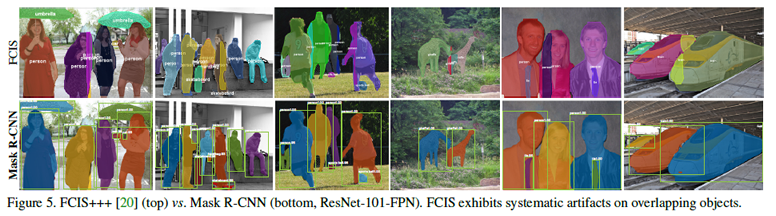
\includegraphics{./img/ch9/figure_9.8_4.png}
%\caption{}
\end{figure}

\section{9.10
CNN在基于弱监督学习的图像分割中的应用}\label{cnnux5728ux57faux4e8eux5f31ux76d1ux7763ux5b66ux4e60ux7684ux56feux50cfux5206ux5272ux4e2dux7684ux5e94ux7528}

  
答案来源:\href{https://zhuanlan.zhihu.com/p/23811946}{CNN在基于弱监督学习的图像分割中的应用}

  
最近基于深度学习的图像分割技术一般依赖于卷积神经网络CNN的训练,训练过程中需要非常大量的标记图像,即一般要求训练图像中都要有精确的分割结果。\\
  
对于图像分割而言,要得到大量的完整标记过的图像非常困难,比如在ImageNet数据集上,有1400万张图有类别标记,有50万张图给出了bounding
box,但是只有4460张图像有像素级别的分割结果。对训练图像中的每个像素做标记非常耗时,特别是对医学图像而言,完成对一个三维的CT或者MRI图像中各组织的标记过程需要数小时。\\
  
如果学习算法能通过对一些初略标记过的数据集的学习就能完成好的分割结果,那么对训练数据的标记过程就很简单,这可以大大降低花在训练数据标记上的时间。这些初略标记可以是:\\
   1、只给出一张图像里面包含哪些物体,\\
   2、给出某个物体的边界框,\\
  
3、对图像中的物体区域做部分像素的标记,例如画一些线条、涂鸦等(scribbles)。

\subsection{9.10.1 Scribble标记}\label{scribbleux6807ux8bb0}

  
论文地址:\href{https://www.cv-foundation.org/openaccess/content_cvpr_2016/papers/Lin_ScribbleSup_Scribble-Supervised_Convolutional_CVPR_2016_paper.pdf}{ScribbleSup:
Scribble-Supervised Convolutional Networks for Semantic Segmentation
(CVPR 2016)}\\
   香港中文大学的Di
Lin提出了一个基于Scribble标记的弱监督学习方法。Scribble是一个很方便使用的标记方法,因此被用得比较广泛。如下图,只需要画五条线就能完成对一副图像的标记工作。

%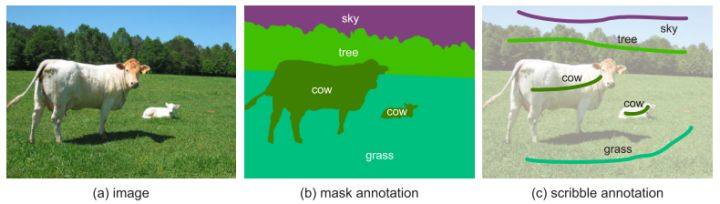
\includegraphics{./img/ch9/figure_9.9_1.png}\\
  
ScribbleSup分为两步,第一步将像素的类别信息从scribbles传播到其他未标记的像素,自动完成所有的训练图像的标记工作;
第二步使用这些标记图像训练CNN。在第一步中,该方法先生成super-pxels,
然后基于graph cut的方法对所有的super-pixel进行标记。

\begin{figure}
\centering
%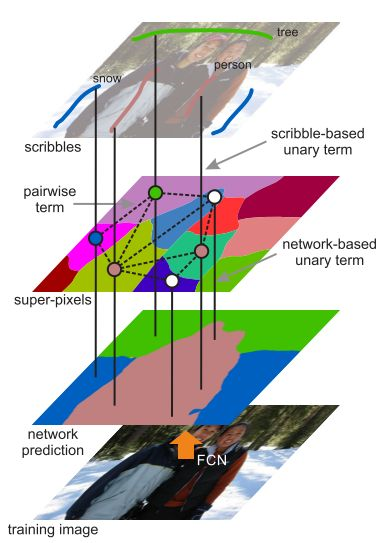
\includegraphics{./img/ch9/figure_9.9_2.png}
%\caption{}
\end{figure}

   Graph Cut的能量函数为:

\[
\sum_{i}\psi _i\left(y_i|X,S\right)+\sum_{i,j}\psi_{ij}\left(y_i,y_j,X\right)
\]

  
在这个graph中,每个super-pixel是graph中的一个节点,相接壤的super-pixel之间有一条连接的边。这个能量函数中的一元项包括两种情况,一个是来自于scribble的,一个是来自CNN对该super-pixel预测的概率。整个最优化过程实际上是求graph
cut能量函数和CNN参数联合最优值的过程:

\[
\sum_{i}\psi _i^{scr}\left(y_i|X,S\right)+\sum _i-logP\left(y_i| X,\theta\right)+\sum_{i,j}\psi _{ij}\left(y_i,y_j|X\right)
\]

   上式的最优化是通过交替求 \(Y\) 和 \(\theta\)
的最优值来实现的。文章中发现通过三次迭代就能得到比较好的结果。

\begin{figure}
\centering
%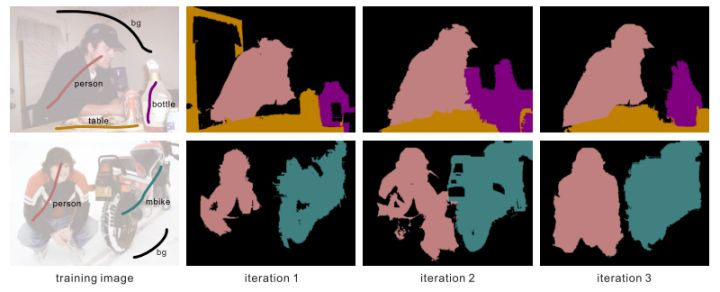
\includegraphics{./img/ch9/figure_9.9_3.png}
%\caption{}
\end{figure}

\subsection{9.10.2
图像级别标记}\label{ux56feux50cfux7ea7ux522bux6807ux8bb0}

  
论文地址:\href{https://www.cv-foundation.org/openaccess/content_iccv_2015/papers/Pathak_Constrained_Convolutional_Neural_ICCV_2015_paper.pdf}{Constrained
Convolutional Neural Networks for Weakly Supervised Segmentation (ICCV
2015)}\\
   UC Berkeley的Deepak
Pathak使用了一个具有图像级别标记的训练数据来做弱监督学习。训练数据中只给出图像中包含某种物体,但是没有其位置信息和所包含的像素信息。该文章的方法将image
tags转化为对CNN输出的label分布的限制条件,因此称为 Constrained
convolutional neural network (CCNN).

%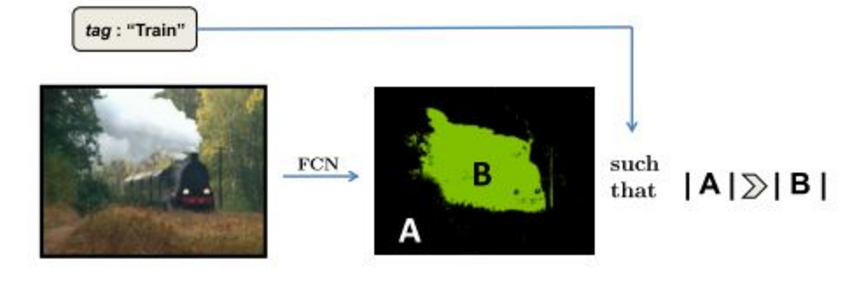
\includegraphics{./img/ch9/figure_9.9_4.png}\\
  

该方法把训练过程看作是有线性限制条件的最优化过程:

\[
\underset{\theta ,P}{minimize}\qquad D(P(X)||Q(X|\theta ))\\
subject\to\qquad A\overrightarrow{P} \geqslant \overrightarrow{b},\sum_{X}^{ }P(X)=1
\]   

其中的线性限制条件来自于训练数据上的标记,例如一幅图像中前景类别像素个数期望值的上界或者下界(物体大小)、某个类别的像素个数在某图像中为0,或者至少为1等。该目标函数可以转化为为一个loss
function,然后通过SGD进行训练。

%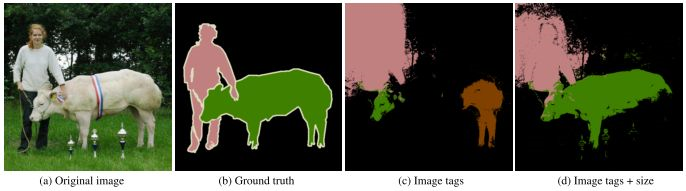
\includegraphics{./img/ch9/figure_9.9_5.png}\\
   实验中发现单纯使用Image
tags作为限制条件得到的分割结果还比较差,在PASCAL VOC 2012
test数据集上得到的mIoU为35.6\%,加上物体大小的限制条件后能达到45.1\%,如果再使用bounding
box做限制,可以达到54\%。FCN-8s可以达到62.2\%,可见弱监督学习要取得好的结果还是比较难。

\subsection{9.10.3 DeepLab+bounding box+image-level
labels**}\label{deeplabbounding-boximage-level-labels}

   论文地址:\href{https://arxiv.org/pdf/1502.02734.pdf}{Weakly-and
Semi-Supervised Learning of a DCNN for Semantic Image Segmentation}\\
   Google的George Papandreou 和UCLA的Liang-Chieh
Chen等在DeepLab的基础上进一步研究了使用bounding box和image-level
labels作为标记的训练数据。使用了期望值最大化算法(EM)来估计未标记的像素的类别和CNN的参数。

%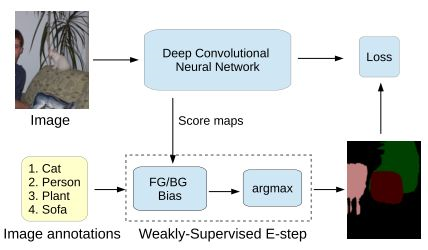
\includegraphics{./img/ch9/figure_9.9_6.png}\\
   对于image-level标记的数据,我们可以观测到图像的像素值和图像级别的标记
,但是不知道每个像素的标号,因此把\(y\)当做隐变量。使用如下的概率图模式:
\[
P\left ( x,y,z;\theta \right ) = P\left ( x \right )\left (\prod_{m=1}^{M} P\left ( y_m|x;\theta \right )\right )P\left ( z|y \right )
\]   
这篇论文是通过EM算法来学习模型的参数\(\theta\),具体推导过程可参考原论文。

%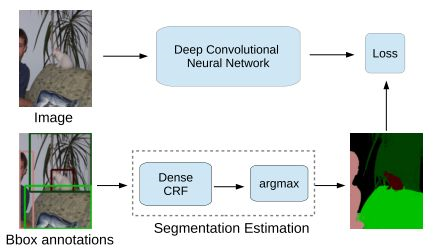
\includegraphics{./img/ch9/figure_9.9_7.png}\\
   对于给出bounding
box标记的训练图像,该方法先使用CRF对该训练图像做自动分割,然后在分割的基础上做全监督学习。通过实验发现,单纯使用图像级别的标记得到的分割效果较差,但是使用bounding
box的训练数据可以得到较好的结果,在VOC2012 test数据集上得到mIoU
62.2\%。另外如果使用少量的全标记图像和大量的弱标记图像进行结合,可以得到与全监督学习(70.3\%)接近的分割结果(69.0\%)。

\subsection{9.10.4 统一的框架}\label{ux7edfux4e00ux7684ux6846ux67b6}

  
论文地址:\href{https://www.cv-foundation.org/openaccess/content_cvpr_2015/papers/Xu_Learning_to_Segment_2015_CVPR_paper.pdf}{Learning
to Segment Under Various Forms of Weak Supervision (CVPR 2015)}

   Wisconsin-Madison大学的Jia
Xu提出了一个统一的框架来处理各种不同类型的弱标记:图像级别的标记、bounding
box和部分像素标记如scribbles。该方法把所有的训练图像分成共计\(n\)个super-pixel,对每个super-pixel提取一个\(d\)维特征向量。因为不知道每个super-pixel所属的类别,相当于无监督学习,因此该方法对所有的super-pixel做聚类,使用的是最大间隔聚类方法(max-margin
clustering, MMC),该过程的最优化目标函数是: \[
\underset{W,H}{min} \qquad  \frac{1}{2}tr\left ( W^TW \right ) + \lambda\sum_{p=1}^{n}\sum_{c=1}^{C}\xi \left ( w_c;x_p;h_p^c \right)
\]

  
在这个目标函数的基础上,根据不同的弱标记方式,可以给出不同的限制条件,因此该方法就是在相应的限制条件下求最大间隔聚类。

\begin{figure}
\centering
%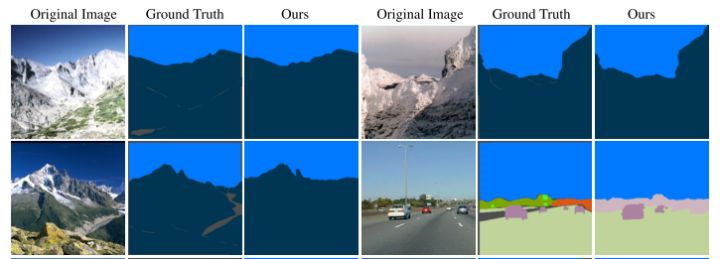
\includegraphics{./img/ch9/figure_9.9_8.png}
%\caption{}
\end{figure}

  
该方法在Siftflow数据集上得到了比较好的结果,比state-of-the-art的结果提高了10\%以上。

  
小结:在弱标记的数据集上训练图像分割算法可以减少对大量全标记数据的依赖,在大多数应用中会更加贴合实际情况。弱标记可以是图像级别的标记、边框和部分像素的标记等。训练的方法一般看做是限制条件下的最优化方法。另外EM算法可以用于CNN参数和像素类别的联合求优。

\subsection{9.10.5
弱监督分割最新进展(贡献者:明奇-北京理工大学)}\label{ux5f31ux76d1ux7763ux5206ux5272ux6700ux65b0ux8fdbux5c55ux8d21ux732eux8005ux660eux5947-ux5317ux4eacux7406ux5de5ux5927ux5b66}

\begin{itemize}
% \tightlist
\item
  \textbf{bbox监督}
\end{itemize}

\begin{enumerate}
\def\labelenumi{\arabic{enumi}.}
% \tightlist
\item
  Learning to Segment via Cut-and-Paste(ECCV 2018)
\end{enumerate}

利用GAN对抗学习的思想,在cut-paste思想指导下利用bbox弱监督进行实例分割。
%\includegraphics{./img/ch9/9.10.5-1.png}\\
采用对抗学习的思想,网络主体分为两大部分:mask生成器和合成图像判别器。具体过程为:(1)在图像上截取gt,经过特征提取后预测一个bbox内gt的mask;(2)在原图上随机cut一个背景图像,将bbox内按照生成的mask提取出物体分割结果,然后paste到原图裁剪的背景上去;(3)合成的图像经过判别器进行真假判断。
通过生成器生成更好mask来使得判别器更难判别,在对抗学习中提升两者的性能,逐渐获得更好的结果
.

\begin{enumerate}
\def\labelenumi{\arabic{enumi}.}
\setcounter{enumi}{1}
% \tightlist
\item
  Simple Does It: Weakly Supervised Instance and Semantic
  Segmentation(CVPR2017)
  本文做的是bbox弱监督语义/实例分割任务,能达到全监督分割效果(DeepLabv1)的95\%。主要工作为:讨论了使用弱监督语义标签进行迭代训练的方法,以及其限制和不足之处;证明了通过类似GrabCut的算法能通过bbox生成分割训练标签方法的可行性,可以避免像上面的迭代方法重新调整网络训练策略;在VOC数据集上逼近监督学习的分割任务效果。
  作者的启发是:将bbox
  level的mask送入网络训练后得到分割mask的比输入的bbox
  mask要好(这是很好的insight)。因此启发的操作是:将bbox
  level标注作为初始mask输入优化,每次得到的标注作为gt进行下一轮的迭代,从而不断获得更好的效果。效果图如下:
  %\includegraphics{./img/ch9/9.10.5-3.png}
  在此基础上,再加上优化的GrabCut+算法,以及部分区域的筛选,以及BSDS500的边界预测信息整合到一起,能够达到很好的弱监督迭代分割效果。
\end{enumerate}

\begin{itemize}
% \tightlist
\item
  \textbf{分类监督}
\end{itemize}

\begin{enumerate}
\def\labelenumi{\arabic{enumi}.}
\item
  Weakly Supervised Learning of Instance Segmentation with Inter-pixel
  Relations(CVPR2019)
  使用分类标注作为弱监督信息,在CAM提取到特征的基础上,进一步设计IRNet学习额外的特征约束,从而到达更好的弱监督实例分割效果。为了解决CAM应用到实例分割的上述局限,设计IRNet。其组成为两部分:(1)不分类别的实例响应图
  (2)pairwise semantic
  affinitie。其中通过不分类别的实例响应图和CAM结合,约束后得到instance-wise
  CAMS;另一个分支预先预测物体的边界然后得到pairwise semantic
  affinitie(关于这个的论文参考Related
  Work的对应部分,有相应的方法,暂时不深究)进行融合和处理得到最终的分割。整体流程如下:
  %\includegraphics{./img/ch9/9.10.5-2.png}
\item
  Weakly Supervised Instance Segmentation using Class Peak
  Response(CVPR2018)
  本文使用图像级的类别标注监督信息,通过探索类别响应峰值使分类网络能够很好地提取实例分割mask。本工作是使用图像级标注进行弱监督实例分割的首个工作。
  在分类监督信息之下,CNN网络会产生一个类别响应图,每个位置是类别置信度分数。其局部极大值往往具有实例很强视觉语义线索。首先将类别峰值响应图的信息进行整合,然后反向传播将其映射到物体实例信息量较大的区域如边界。上述从类别极值响应图产生的映射图称为Peak
  Response Maps
  (PRMs),该图提供了实例物体的详细表征,可以很好地用作分割监督信息。
  具体流程如图: %\includegraphics{./img/ch9/9.10.5-4.png}
  首先将图片经过正常的分类网络训练,其中在类别预测响应图上提取出局部响应极值点,进行增强卷积后预测出PRM。然后结合多种信息进行推断生成mask。
\item
  Weakly Supervised Semantic Segmentation Using Superpixel Pooling
  Network(AAAI 2017)
  本文介绍通过类别标注的标签实现弱监督语义分割的方法。该方法在语义分割mask生成和使用生成mask学习分割生成网络之间反复交替。要实现这种交替迭代学习,关键点就是如何利用类别标注得到较准确的初始分割。为了解决这一问题,提出了Superpixel
  Pooling Network
  (SPN),将输入图像的超像素分割结果作为低阶结构的表征,辅助语义分割的推断。
  %\includegraphics{./img/ch9/9.10.5-5.png}
  首先是SPN生成初始mask,然后用另一个网络DecoupledNet来学习每个像素的mask标注。其中,该分割网络将语义分割任务解耦为分类和分割两个子任务,并且能够从类别标注中学习形状先验知识用于辅助分割。
\end{enumerate}

\section{9.11
DenseNet(贡献者:黄钦建-华南理工大学)}\label{densenetux8d21ux732eux8005ux9ec4ux94a6ux5efaux534eux5357ux7406ux5de5ux5927ux5b66}

   这篇论文是CVPR2017年的最佳论文。

  
卷积神经网络结构的设计主要朝着两个方向发展,一个是更宽的网络(代表:GoogleNet、VGG),一个是更深的网络(代表:ResNet)。但是随着层数的加深会出现一个问题------梯度消失,这将会导致网络停止训练。到目前为止解决这个问题的思路基本都是在前后层之间加一个identity
connections(short path)。

\begin{figure}
\centering
%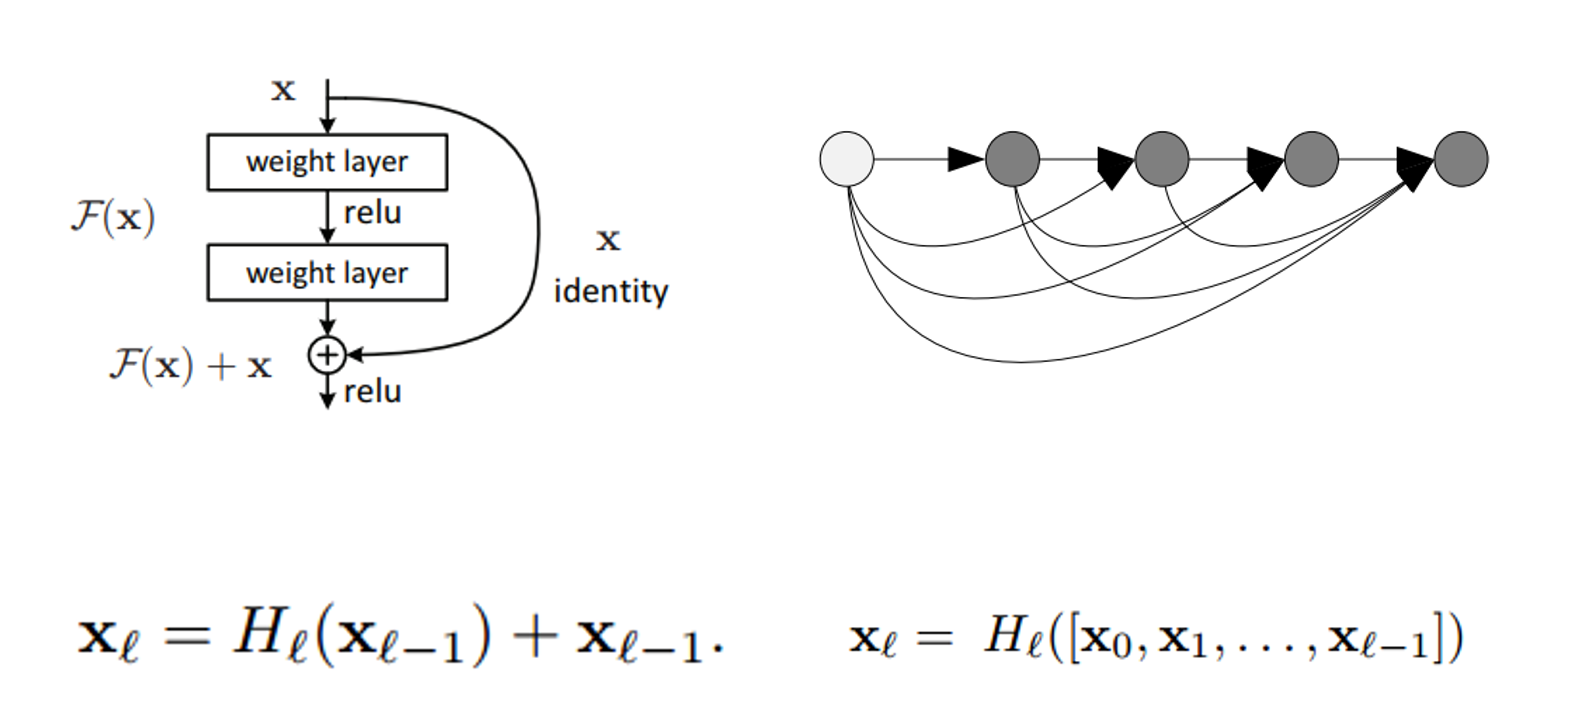
\includegraphics{./img/ch9/9-10-3.png}
%\caption{}
\end{figure}

  
由上图中可知Resnet是做值的相加(也就是add操作),通道数是不变的。而DenseNet是做通道的合并(也就是Concatenation操作),就像Inception那样。从这两个公式就可以看出这两个网络的本质不同。此外DensetNet的前面一层输出也是后面所有层的输入,这也不同于ResNet残差网络。

\begin{figure}
\centering
%\includegraphics{./img/ch9/9-10-1.png}
%\caption{}
\end{figure}

   DenseNet的Block结构如上图所示。

  
1*1卷积核的目的:减少输入的特征图数量,这样既能降维减少计算量,又能融合各个通道的特征。我们将使用BottleNeck
Layers的DenseNet表示为DenseNet-B。(在论文的实验里,将1×1×n小卷积里的n设置为4k,k为每个H产生的特征图数量)

\begin{figure}
\centering
%\includegraphics{./img/ch9/9-10-2.png}
%\caption{}
\end{figure}

  
上图是DenseNet网络的整体网络结构示意图。其中1*1卷积核的目的是进一步压缩参数,并且在Transition
Layer层有个参数Reduction(范围是0到1),表示将这些输出缩小到原来的多少倍,默认是0.5,这样传给下一个Dense
Block的时候channel数量就会减少一半。当Reduction的值小于1的时候,我们就把带有这种层的网络称为DenseNet-C。

   DenseNet网络的优点包括: - 减轻了梯度消失 - 加强了feature的传递 -
更有效地利用了feature~ - 一定程度上较少了参数数量 -
一定程度上减轻了过拟合

\section{9.12
图像分割的常用数据集}\label{ux56feux50cfux5206ux5272ux7684ux5e38ux7528ux6570ux636eux96c6}

\subsection{9.12.1 PASCAL VOC}\label{pascal-voc}

VOC 数据集分为20类,包括背景为21类,分别如下: - Person: person -
Animal: bird, cat, cow, dog, horse, sheep - Vehicle: aeroplane, bicycle,
boat, bus, car, motorbike, train - Indoor: bottle, chair, dining table,
potted plant, sofa, tv/monitor

VOC
数据集中用于分割比赛的图片实例如下,包含原图以及图像分类分割和图像物体分割两种图(PNG格式)。图像分类分割是在20种物体中,ground-turth图片上每个物体的轮廓填充都有一个特定的颜色,一共20种颜色。

\begin{figure}
\centering
%\includegraphics{./img/ch9/VOC-01.png}
%\caption{}
\end{figure}

\subsection{9.12.2 MS COCO}\label{ms-coco}

MS COCO 是最大图像分割数据集,提供的类别有 80 类,有超过 33
万张图片,其中 20 万张有标注,整个数据集中个体的数目超过 150 万个。MS
COCO是目前难度最大,挑战最高的图像分割数据集。

\begin{figure}
\centering
%\includegraphics{./img/ch9/COCO-01.png}
%\caption{}
\end{figure}

\subsection{9.12.3 Cityscapes}\label{cityscapes}

Cityscapes
是驾驶领域进行效果和性能测试的图像分割数据集,它包含了5000张精细标注的图像和20000张粗略标注的图像,这些图像包含50个城市的不同场景、不同背景、不同街景,以及30类涵盖地面、建筑、交通标志、自然、天空、人和车辆等的物体标注。Cityscapes评测集有两项任务:像素级(Pixel-level)图像场景分割(以下简称语义分割)与实例级(Instance-level)图像场景分割(以下简称实例分割)。

\begin{figure}
\centering
%\includegraphics{./img/ch9/Cityscapes-01.png}
%\caption{}
\end{figure}

\section{9.13
全景分割(贡献者:北京理工大学--明奇)}\label{ux5168ux666fux5206ux5272ux8d21ux732eux8005ux5317ux4eacux7406ux5de5ux5927ux5b66ux660eux5947}

全景分割的开山之作:何恺明的\emph{Panoptic Segmentation}

\begin{enumerate}
\def\labelenumi{\arabic{enumi}.}
% \tightlist
\item
  \textbf{Introduction}
\end{enumerate}

  语义分割通过带孔全卷积网络,根据不同的stuff进行划分;实例分割则是在目标检测的基础上基于检测框进行物体的分割。缺少一种框架可以将两者进行融合实现既能分割背景又能分割实例,而这在自动驾驶和AR技术中大有作为。由此提出的全景分割任务能将两者进行结合。

  全景分割的思路很直观:为图像的每个像素分配语义label和类内实例id,前者用于区分语义信息,后者用于分割实例(因此stuff不具有实例id)。提出全景分割时,只是启发式地将语意分割和实例分割两种任务的输出进行后处理的融合(如NMS),并以此建立PS任务的baseline。为了评价全景分割的质量,提出panoptic
quality (PQ) 标准,将背景和物体的评价纳入一个完整的框架下。示意图如下:
%\includegraphics{./img/ch9/9.13-1.png}

\begin{enumerate}
\def\labelenumi{\arabic{enumi}.}
\setcounter{enumi}{1}
% \tightlist
\item
  \textbf{Panoptic Segmentation}
\end{enumerate}

\begin{itemize}
\item
  \textbf{Task format}\\
  全景分割的标注方法:\\
  像素级的标注,标出类别label和类内实例id。如果某像素的这两个信息都能匹配,则可以将该像素匹配到某个类别和实例中去;类外的像素可以分配空标签,即并不是所有的像素都要有语义类别。
\item
  \textbf{Stuff and thing labels}\\
  对于stuff和thing(背景填充和物体实例)的标签,交集是空集,并集是所有可能的label空间。这两者是互相独立不相关的(很好理解,像素属于那个类和它属于哪个物体不具有相关性)。
\item
  \textbf{Relationship}\\
  都是像素级的label,需要为每个像素分配对应的标签。但是实例分割基于region的,允许重叠的segmentation,而全景分割和语义分割一样是像素级的label,不允许重叠标签的出现。
\item
  \textbf{Confidence scores}\\
  这一点上更像语义分割而不是实例分割,对于PS不需要置信分数评价分割质量。提到这个,作者认为语义分割和全景分割可以直接利用人工标注的label进行对比从而评价当前mask的质量;而实例分割在选择mask时评价的是分类置信度,这个并没有人工标注进行参考,因此难以把握。
\end{itemize}

\begin{enumerate}
\def\labelenumi{\arabic{enumi}.}
\setcounter{enumi}{2}
% \tightlist
\item
  \textbf{Panoptic Segmentation Metric}\\
    用于衡量全景分割效果的指标应具有:完备性;可解释性;简洁性。由是提出了PQ指标,可分为两步:分割匹配、在匹配上进行计算PQ。
\end{enumerate}

3.1 \textbf{Segment Matching}\\
  定义match:预测的segmentation和gt的iou大于0.5,说明两者can
match。再结合全景分割的不可重叠性,不难得到:最多只有一个预测的segmentation可以match
gt。

3.2 \textbf{PQ Computation}\\
  PQ的计算类似mAP,也是类内求取,然后求类间的平均值,以便不敏感类别不平衡。对于每一类,可以根据gt与预测的segmentation分为三类(下图描述):
%\includegraphics{./img/ch9/9.13-2.png}

TP: 预测为正,实际为正,描述match较好的\\
FP: 预测为正,实际为负,描述match错的\\
FN: 预测为负,实际为正,描述没match出来的gt\\
  通过上述三类可以计算得到PQ值公式:
%\includegraphics{./img/ch9/9.13-3.png}

式中出去FP与FN后,剩下的式子描述的是match的segmentation的平均IoU,加上FP与FN是为了惩罚match失败的分割实例。\\
有意思的是,对上述式子进行简单的恒等变化:
%\includegraphics{./img/ch9/9.13-4.png}

第一项评价的是match分割的质量,第二项类似于F1得分。因此可以PQ分解为:\\
\[PQ=SQ*RQ\]

\begin{itemize}
\item
  \textbf{Void labels}\\
  gt中可能出现两种像素标注为空的情况:超出类别的像素和模糊不清的像素(难以分类)。在评估结果时,这些空的标签不予以评估。具体而言:\\
  (1)在matching部分,预测出为void的像素会被移出prediction并不参与IoU计算;\\
  (2)matching后,unmatched prediction按照一般情况会计算FP
  FN,但是对于空标签情况,如果该prediction含有的void像素块超过一定匹配阈值就会被移除,并不算作FP计算得分。
\item
  \textbf{Group labels}\\
  有时区分相同语义类别的实例个体标注比较困难,因此有提出组标签的标注方法。但对于PQ计算而言:\\
  (1)matching部分不使用组标签,而是严格区分实例\\
  (2)matching后,对于包含一部分相同类别像素点的unmatched predicted
  segments,这一部分将被去除并不视作false positives
\end{itemize}

3.3 \textbf{Comparison to Existing Metrics} * \textbf{Semantic
segmentation metrics}\\
衡量语义分割的标准有像素级精度,平均精度,IoU。但是其只专注于像素级的划分,不能反映物体实例级别的分割性能。

\begin{itemize}
\item
  \textbf{Instance segmentation metrics}\\
  度量为AP,主要是引入了置信度分数confidence
  score对检测目标进行打分。(两者不是完全的隔绝,实例分割也有用IoU监督的,而confidence
  score是否能够反映mask的真实质量也有存疑过,这个标准也不是固定的)
\item
  \textbf{Panoptic quality}\\
  PQ的度量可以分解成SQ和RQ,SQ反映了语义分割的像素级IoU性能,RQ专注于检测识别的效果,因此将两者统一到一个框架下。
\end{itemize}

分割效果: %\includegraphics{./img/ch9/9.13-5.png}

TODO

\begin{itemize}
% \tightlist
\item
  图像分割数据集标注工具
\item
  图像分割评价标准
\item
  全景分割
\item
  UNet++
\end{itemize}
